\chapter{Evaluaciones y análisis de resultados}
\label{results}

\section{Parámetros de ejecución}

Todas las evaluaciones se realizaron con los parámetros estándar del método descritos en el manual (ver capítulo \ref{manual}).
%El equipamiento y software utilizado para las pruebas se encuentra descrito en el apéndice \ref{equipamiento}.
El equipamiento y software utilizado para las pruebas es el siguiente:

% Para realizar las pruebas se utilizó el siguiente equipamiento:

\begin{center}
\begin{description}
 \item[Sistema operativo:] Ubuntu 14.04 - Kernel version: 3.13.0
\item[CPU:] Intel(R) Core(TM) i7-4770 CPU @ 3.40GHz
\item[Memoria RAM:] 16GB
\end{description}
\end{center}
% \end{itemize}



\section{Estimación del parámetro $\beta$}\label{betaResults}
% PRIMERO EXPLICAR COMO DEPENDE LA EJECUCION CON EL PARÁMETRO BETA
% PARA VALORES MAS CHICOS ...
% PARA VALORES MAS GRANDES...
% DAR UNA IDEA DEL RANGO DE VALORES BETA DE ACUERDO A LA ECUACION, PARA DIFERENCIAS DE SCORE = 1
% MOSTRAR GRAFICO/S DE RELACION ENTRE 
% POR LO TANTO, UN PARAMETRO QUE TIENE EN CUENTA ESTOS ASPECTOS, QUE PODRIA EVALUAR CORRECTAMENTE LA EJECUCION EN FUNCION DE BETA , Y QUE ADEMAS ES EL DATO MAS IMPORTANTE EN LA EJECUCION ES EL TIEMPO DE EJECUCION

En las secciones previas hemos propuesto un método de diseño que se basa en búsqueda estocástica sobre el espacio de secuencias.
El método de búsqueda es guiado por el resultado de una función que asigna un puntaje a cada secuencia, el cual resulta siempre mayor o igual a 0.
La secuencia resultante buscada se caracteriza por tener un puntaje igual a 0. Por lo tanto, el método puede verse como la búsqueda de un mínimo global sobre la superficie
que relaciona cada posible secuencia con su valor de puntaje.
% El el valor(o el rango) óptimo para el parámetro que Beta depende en gran parte de las características de esta superficie.

El comportamiento del método de búsqueda depende de un único parámetro $\beta$ cuyo valor (o rango) óptimo está fuertemente asociado a las características de esta superficie.
Un valor de $\beta$ más grande tiene un porcentaje de aceptación mayor de mutaciones que aumentan el puntaje de la secuencia. Por lo tanto, permite la exploración de superficies que 
requieren superar mínimos locales para alcanzar secuencias con puntaje 0.
Un valor de $\beta$ más chico implica recorrer un camino más directo hacia el mínimo ya que se aceptan menos mutaciones que aumenten el puntaje, pero esto podría requerir la evaluación de una gran cantidad de posibilidades. 
Incluso, si la búsqueda se estanca en un mínimo local, un valor muy chico de $\beta$ solo podría encontrar la solución en un tiempo muy grande. Como vimos en el capítulo 2, la decisión de aceptación está basada en el uso de la ecuación \ref{monteCarlo}, la cual siempre devuelve un valor $>0$ para cualquier $\beta$ positivo.
% Para cualquier valor de $\beta$ positivo dadas las propiedades del método de decisión para aceptar las mutaciones,   el valor de la ecuación \ref{monteCarlo} siempre será mayor que 0. 
Por lo tanto, la probabilidad de aceptación nunca es 0 y no es imposible encontrar el resultado si es que existe, aún cuando el tiempo que se demore sea demasiado largo para un uso práctico del método.

% En esta aplicación, además, partiendo de una secuencia inicial dada por el usuario, resultaría mejor obtener la secuencia con puntaje mínimo que esté más cerca en la superficie, es decir, que sea más similar a la secuencia inicial.
% Esto implica una menor cantidad de mutaciones, lo que equivale a un valor de beta mas chico.

A pesar que, previo a desarrollar la aplicación asumimos que el espacio de soluciones era considerablemente grande, no sabemos cómo es exactamente 
la superficie que asocia cada secuencia con el puntaje definido por las evaluaciones. 
De esta forma, inicialmente no tenemos ningún conocimiento de cómo se relaciona el valor del parámetro $\beta$ con la ejecución
resultante, ni cuáles serán los valores de $\beta$ que nos permitirán obtener diseños de la forma más eficiente.
% Sin embargo, no sabemos como estos intentos de encontrar mejores mutaciones afectan a la optimalidad de la búsqueda global.
% Para tener una primera idea global de esta dependencia analizamos e
% Todavía no sabemos las implicancias de realizar esta cantidad de intentos de mutacion sobre la búsqueda.
La forma más directa de conocer cuál es el rango (o valor) óptimo de $\beta$ es mediante la evaluación del tiempo de ejecución, es decir, el tiempo total requerido para la búsqueda del diseño resultante. 
Para esto, se midió el tiempo de ejecución para distintas corridas que utilizan valores de $\beta$ en el rango 0.1-2.5.
% La evaluación realizada implicó la medición del tiempo de ejecución para distintas ejecuciones que utilizan valores de beta en el rango 0.1-2.5.
Puntualmente se analizan los valores en el conjunto (0.1, 0.5, 1.0, 1.5, 2.0, 2.3, 2.5). 
Se realizaron 6 ejecuciones para cada valor de $\beta$ analizado, de las cuales 3 se realizan a partir de secuencias definidas (obtenidas de proteínas naturales) y otras 3 a partir de secuencias generadas aleatoriamente.
En todos los casos con una longitud de 50 residuos.

En la figura \ref{fig:beta-vs-time} se muestran los tiempos medios asociados a cada conjunto de evaluaciones.
En primer lugar vemos que no hay una diferencia significativa constante entre las ejecuciones que inician a partir de secuencias naturales y las que lo hacen a partir de secuencias aleatorias.
% Al parecer, si bien las primeras pueden tener valores de score mayore
Por otro lado, se ve que el tiempo de ejecución es altamente variable para la mayoría de los valores de $\beta$.
Esta variabilidad, que se basa en las propiedades estocásticas de la búsqueda, no permite definir un valor óptimo puntual. Se puede ver, igualmente, que el tiempo de ejecución es significativamente mayor en el caso de $\beta$ muy grande (2.3 y 2.5), 
indicando que el rango óptimo de valores está ubicado hacia el extremo inferior.
Aunque el rango completo 0.1-2.0 es aceptable, definimos a $\beta=$1.0 como un valor que nos permitirá realizar la ejecución en un tiempo aceptable, quedando como valor estándar de la herramienta.



\begin{figure}[htbp]
% \advance\leftskip-1.2cm
% 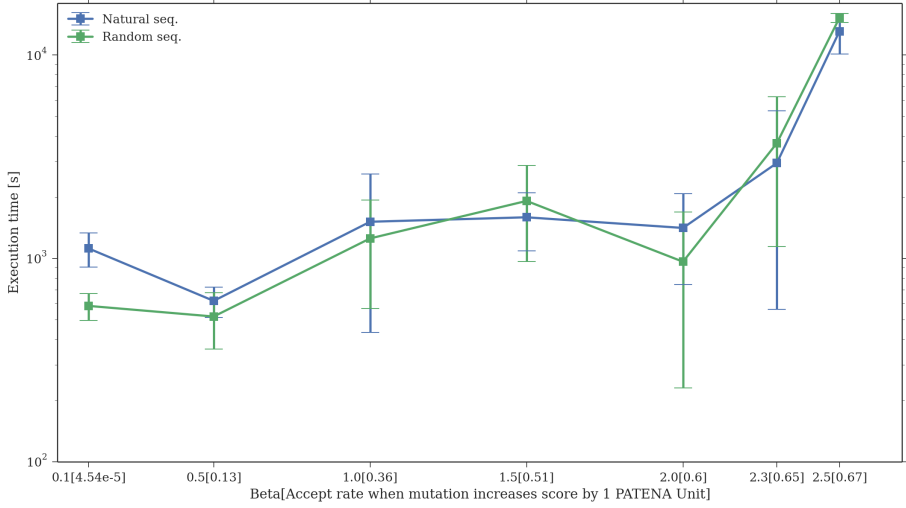
\includegraphics[width=1.1\textwidth]{img/resultados/beta-vs-time-length50-rate.png}
\centering
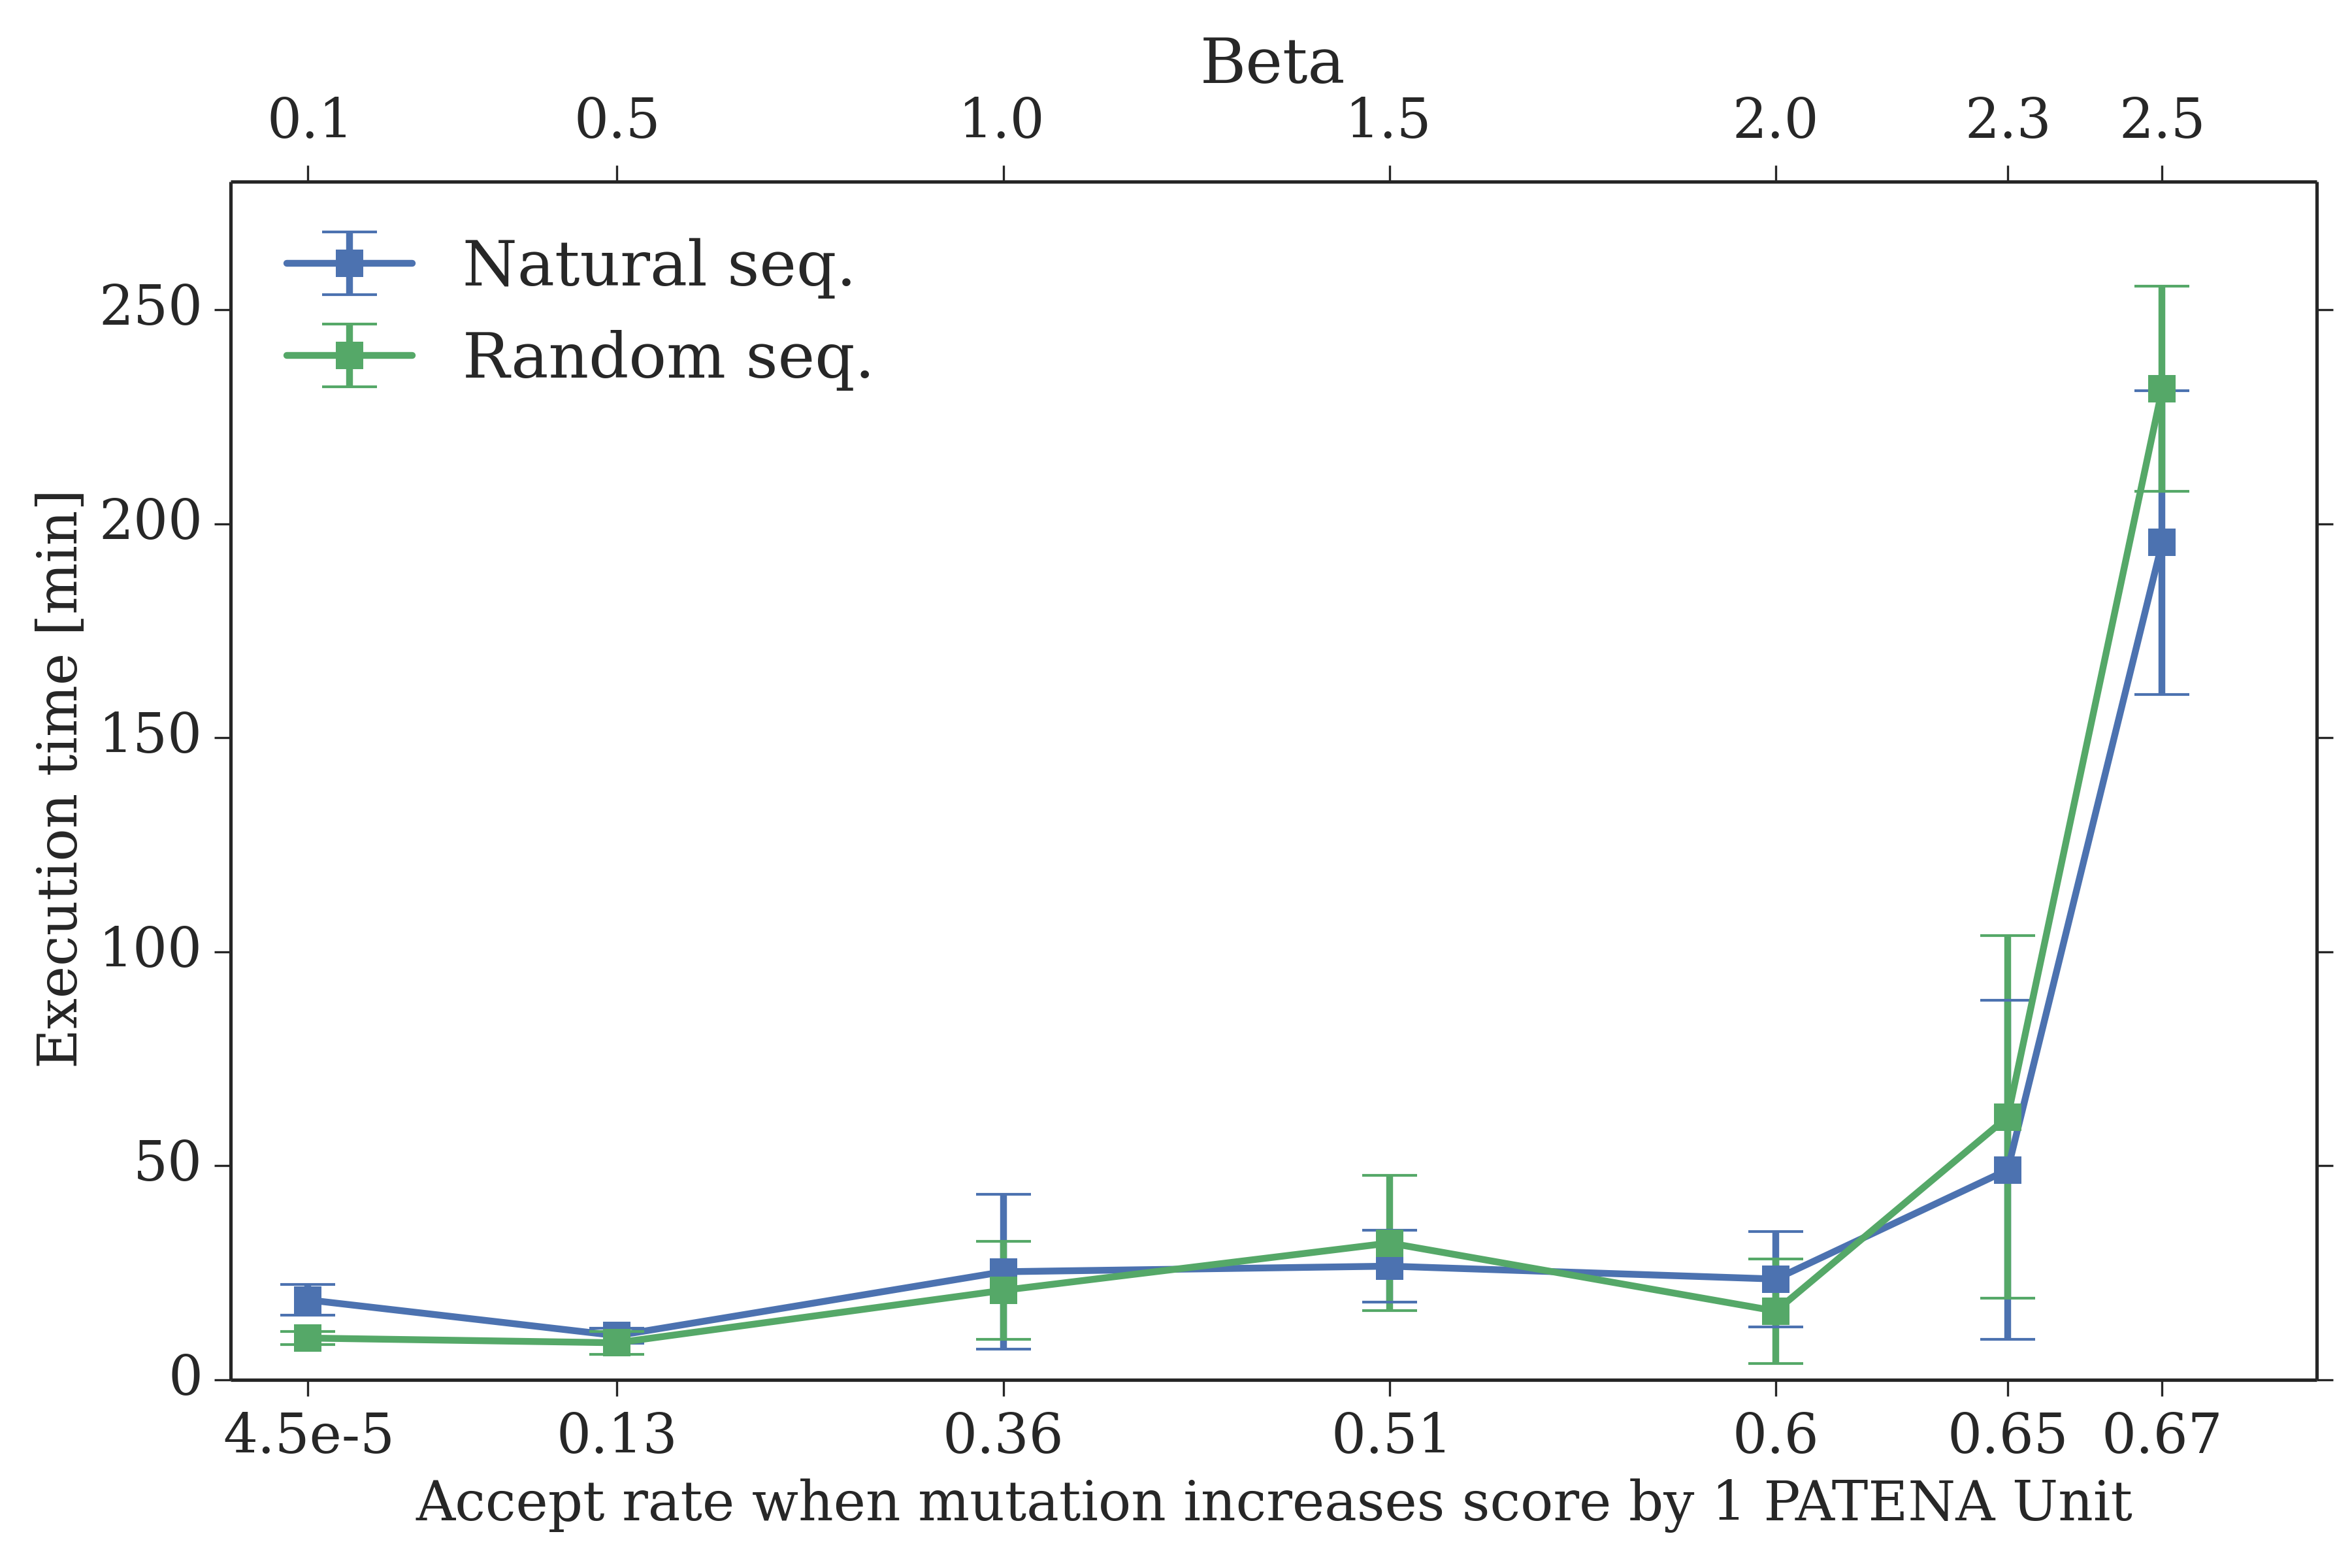
\includegraphics[width=0.9\textwidth]{img/resultados/beta-vs-time-length50-300dpi.png}
\caption{\textbf{Dependencia del tiempo de ejecución con $\beta$}}
\label{fig:beta-vs-time}
\end{figure}



%************************ HASTA ACA ESTA BIEN ***********************












\section{Análisis detallado de la ejecución}
% ***************************************************************
% 
%    ACA LA IDEA ES DESGLOSAR LA DEPENDENCIA DEL TIEMPO CON BETA
% 



% Una vez definido el valor efectivo de $\beta$ queda completo el método listo para su utilización. 
% La estimación del valor de $\beta$ que provea un menor tiempo de ejecución nos permite conocer cual es el valor que provee un correcto balance entre la exploración y la explotación de la superficie.
El rango de $\beta$ obtenido es útil para poder encontrar resultados eficientemente. No obstante, si queremos conocer más en detalle las propiedades de la búsqueda,
% detalle más sobre la superficie que estamos explorando, 
% pero para tener una idea más detallada del perfil de las ejecuciones, 
hace falta desglosar la ejecución.
Los detalles de las búsquedas permiten, además, inferir ciertas características de la superficie que se está explorando.
Sabiendo que las propiedades de la búsqueda son, puntualmente, 
% Sabiendo que los tiempos de ejecución son producto directo de 
la cantidad total de mutaciones aceptadas y la cantidad de mutaciones que se intentan para cada ejecución, 
en lo que resta de esta sección analizaremos cómo cambian los perfiles de estas variables según el valor de $\beta$. % en la búsqueda que estamos realizando.
% Sabemos que el tiempo de ejecución resultante es producto del número de mutaciones y de intentos de mutación, 
 
Para tener una primera idea de esta dependencia, analizaremos los perfiles de ejecución para dos valores puntuales de $\beta$: $\beta=$0.5 y $\beta=$2.4.
En el caso del $\beta$ más chico (0.5), la probabilidad de aceptar una mutación para un incremento de 1 en el puntaje es de $13\%$, mientras que para el $\beta$ más grande (2.4) esta probabilidad es de $65,9\%$.
Por lo tanto, los dos valores podrían clasificarse como cercanos a los extremos dentro del esquema de decisión basado en el puntaje.
Para cada valor de $\beta$ se realizaron 6 corridas independientes.
% En los gráficos \ref{fig:scoreVsiter} y \ref{fig:mutAttemptsVsite} se muestran los resultados de 6 corridas independientes para cada uno de los valores de $\beta$ evaluados (0.5 y 2.4).
% El tiempo de ejecución resultante es producto de dos variables de l
La mitad de estas corridas se iniciaron a partir de secuencias generadas aleatoriamente, mientras que las restantes se inician a partir de secuencias naturales definidas (distintas entre si).
En todos los casos la longitud de la secuencia fue de 30 aminoácidos. Los resultados se muestran en las figuras \ref{fig:scoreVsiter} y \ref{fig:mutAttemptsVsite}.
% donde se muestra el puntaje y los intentos de mutación (respectivamente) frente al número de mutación .
% Este mismo esquema de 6 corridas se repitió para los dos valores de $\beta$ (0.5 y 2.4).
% En el caso del $\beta$ más chico (0.5), la probabilidad de aceptar una mutación para un incremento de 1 en el puntaje es de $13\%$, mientras que para el beta más grande (2.4) esta probabilidad es de $65,9\%$.
% Por lo tanto, los dos valores podrían clasificarse como cercanos a los extremos dentro del esquema de decisión basado en el puntaje.
% rango de posibles valores para $\beta$.
% Los resultados de las corridas se muestran en la tabla ......... ***CONVIENE RESUMIR BIEN LOS DATOS EN UNA TABLA? EL UNICO DATO CREO QUE SERIA EL TOTAL DE ITERACIONES




% 
% \begin{figure} 
% \advance\leftskip-2cm
% \subfigure[Ejecuciones individuales]{\label{fig:scoreVsiter-a}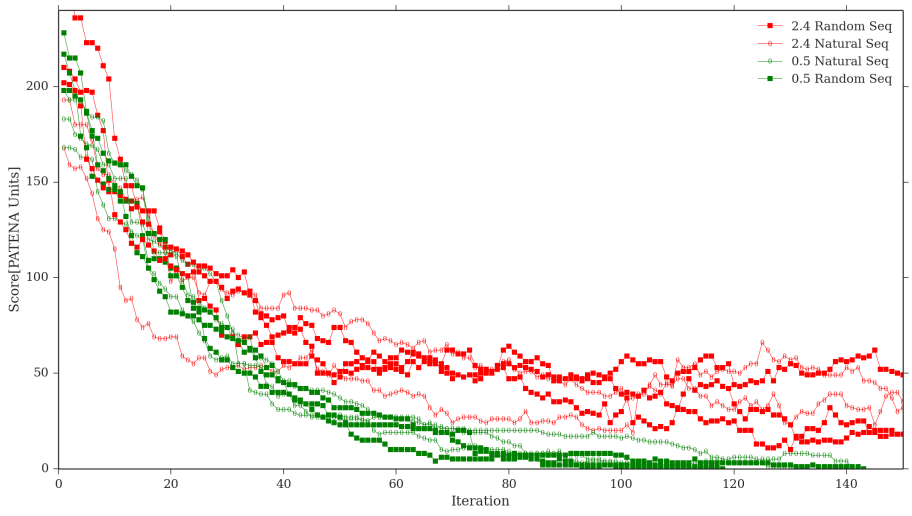
\includegraphics[width=1.15\textwidth]{img/resultados/individuales-scoreVsiter-hasta150.png}}
% \subfigure[Valores medios y desviaciones]{\label{fig:scoreVsiter-b}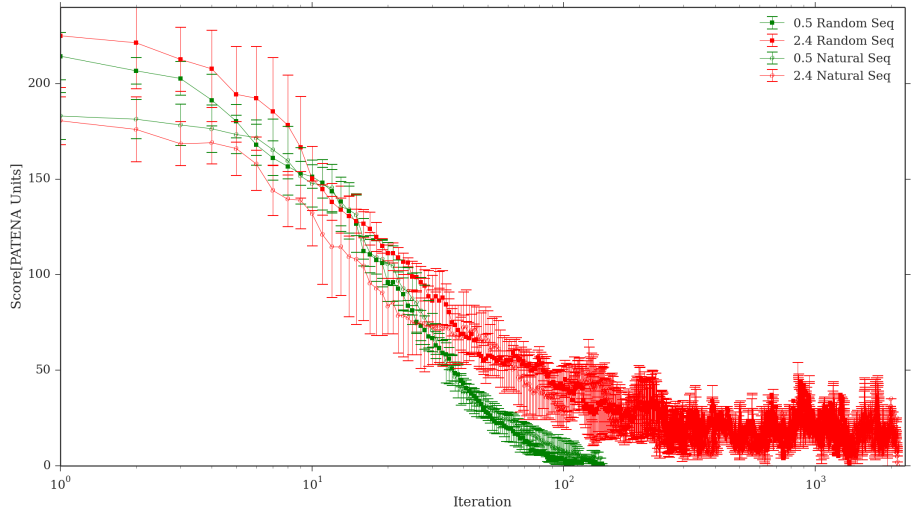
\includegraphics[width=1.15\textwidth]{img/resultados/scoreVsiter-cada1-hasta2270.png}}
%  \caption{Puntaje asociado a cada iteración}
%  \label{fig:scoreVsiter}
% 
% \end{figure}

% SCORE vs MUTACIONES  
\begin{figure}[htbp]
% \advance\leftskip-1.5cm
  \begin{subfigure}[b]{\textwidth}
%     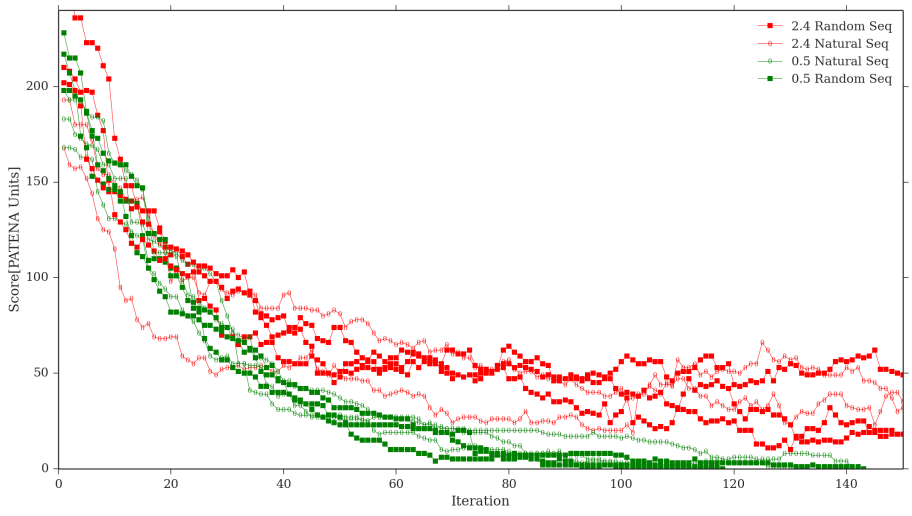
\includegraphics[width=1.15\textwidth]{img/resultados/individuales-scoreVsiter-hasta150.png}
 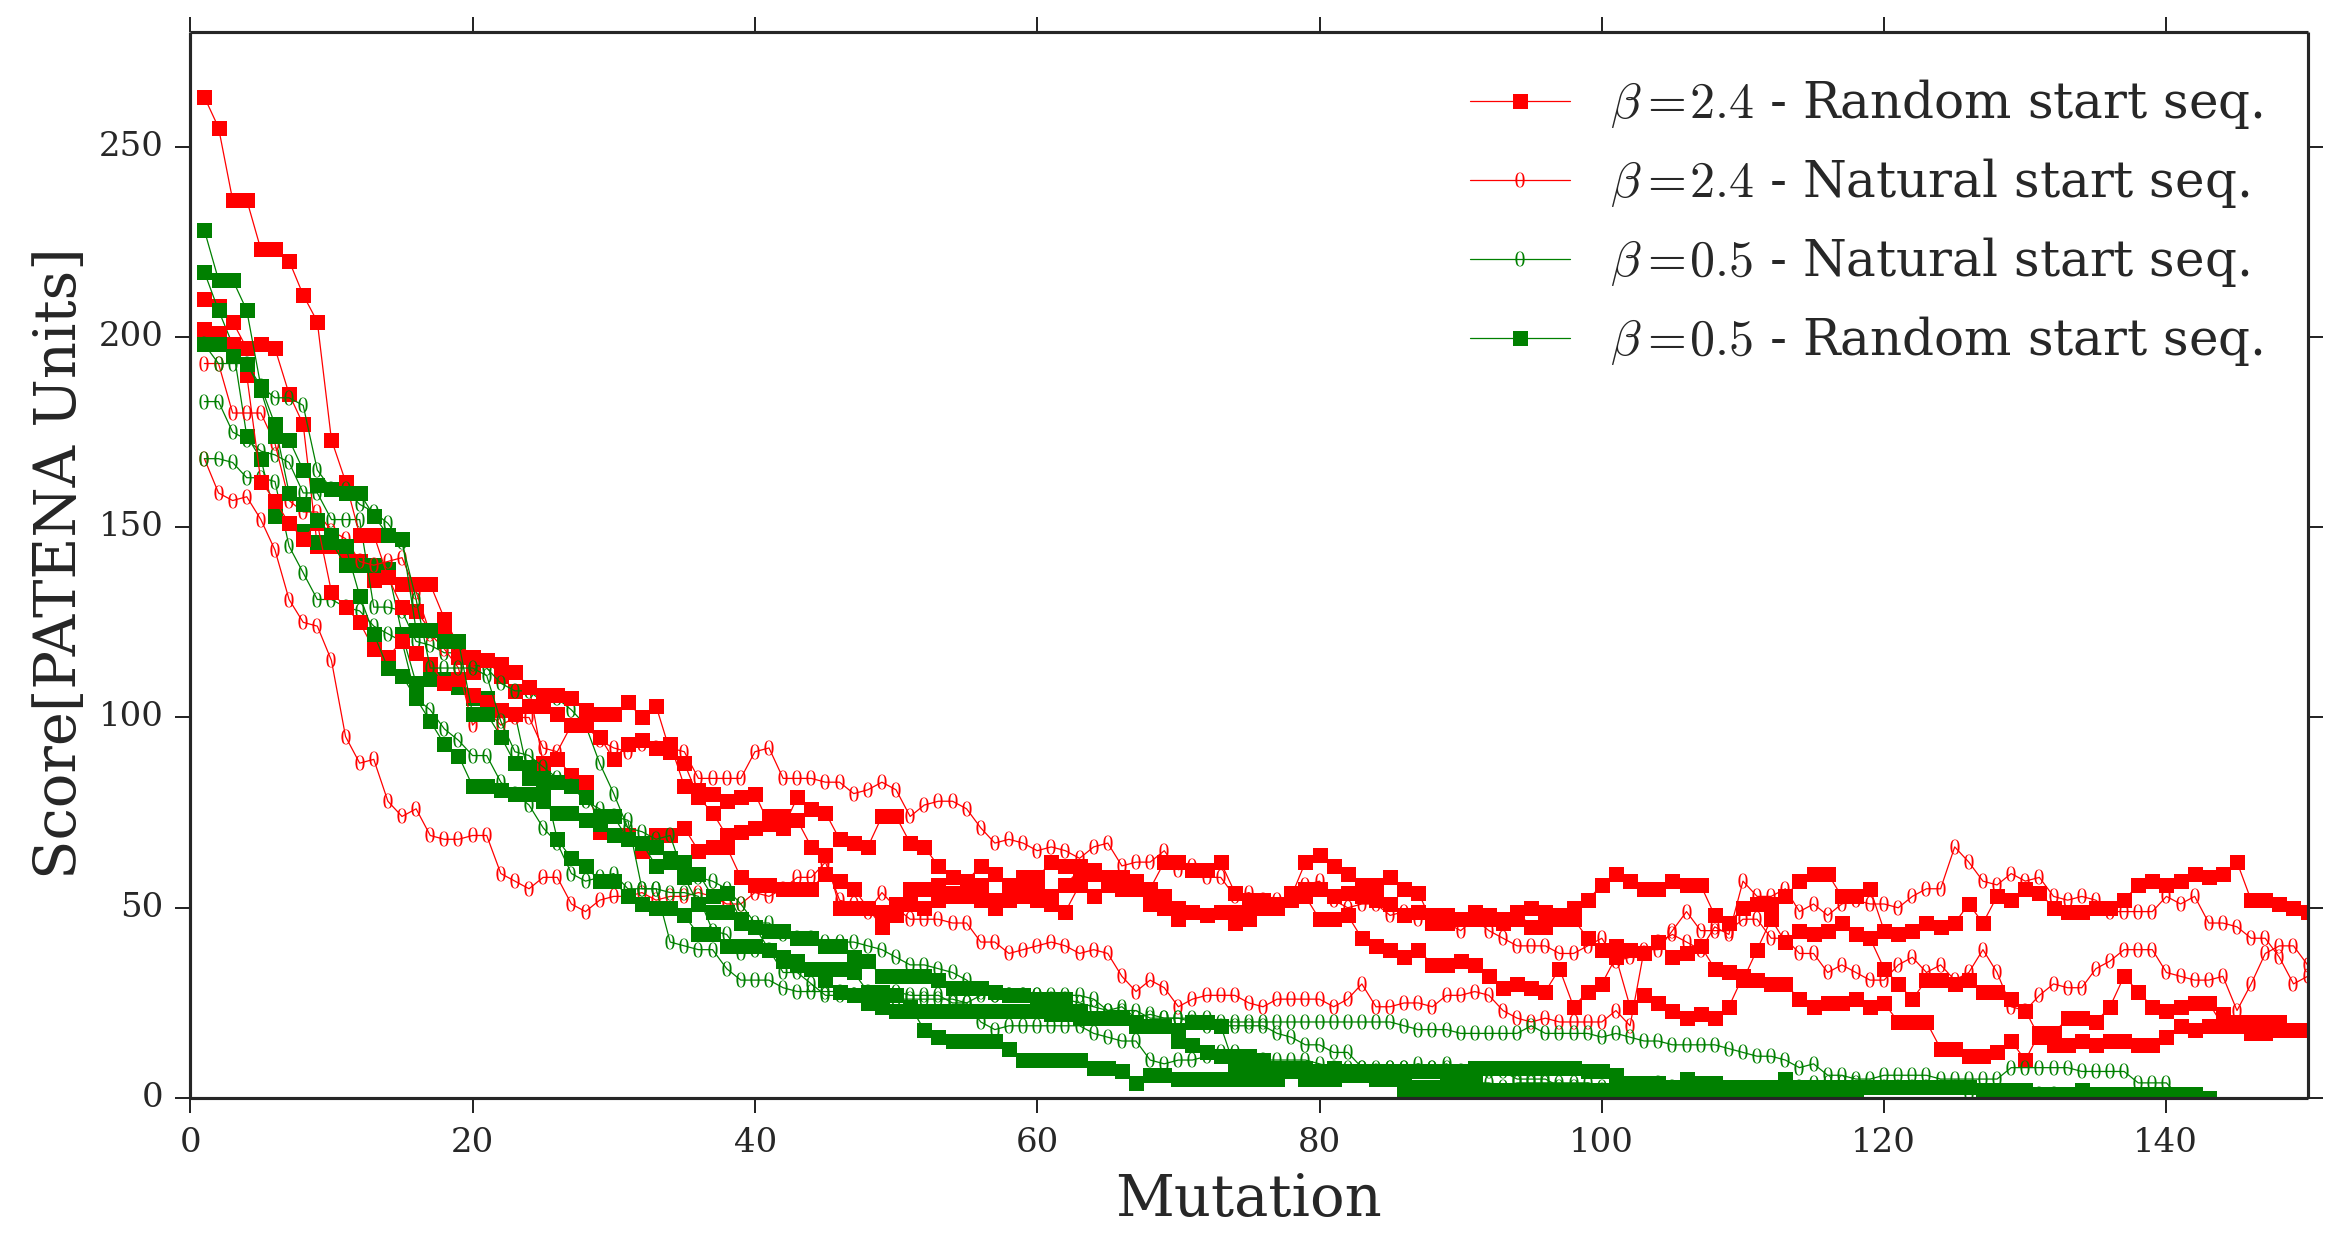
\includegraphics[width=\textwidth]{img/resultados/iterationVsScore-individual.png}
    \caption{Ejecuciones individuales}
    \label{fig:scoreVsiter-a}
  \end{subfigure}
%   \hspace{20px}
  \begin{subfigure}[b]{\textwidth}
%     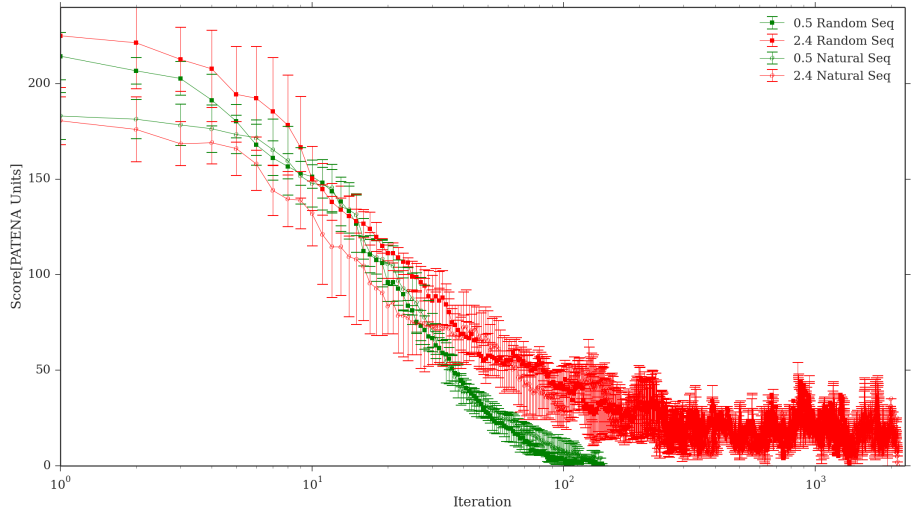
\includegraphics[width=1.15\textwidth]{img/resultados/scoreVsiter-cada1-hasta2270.png}
     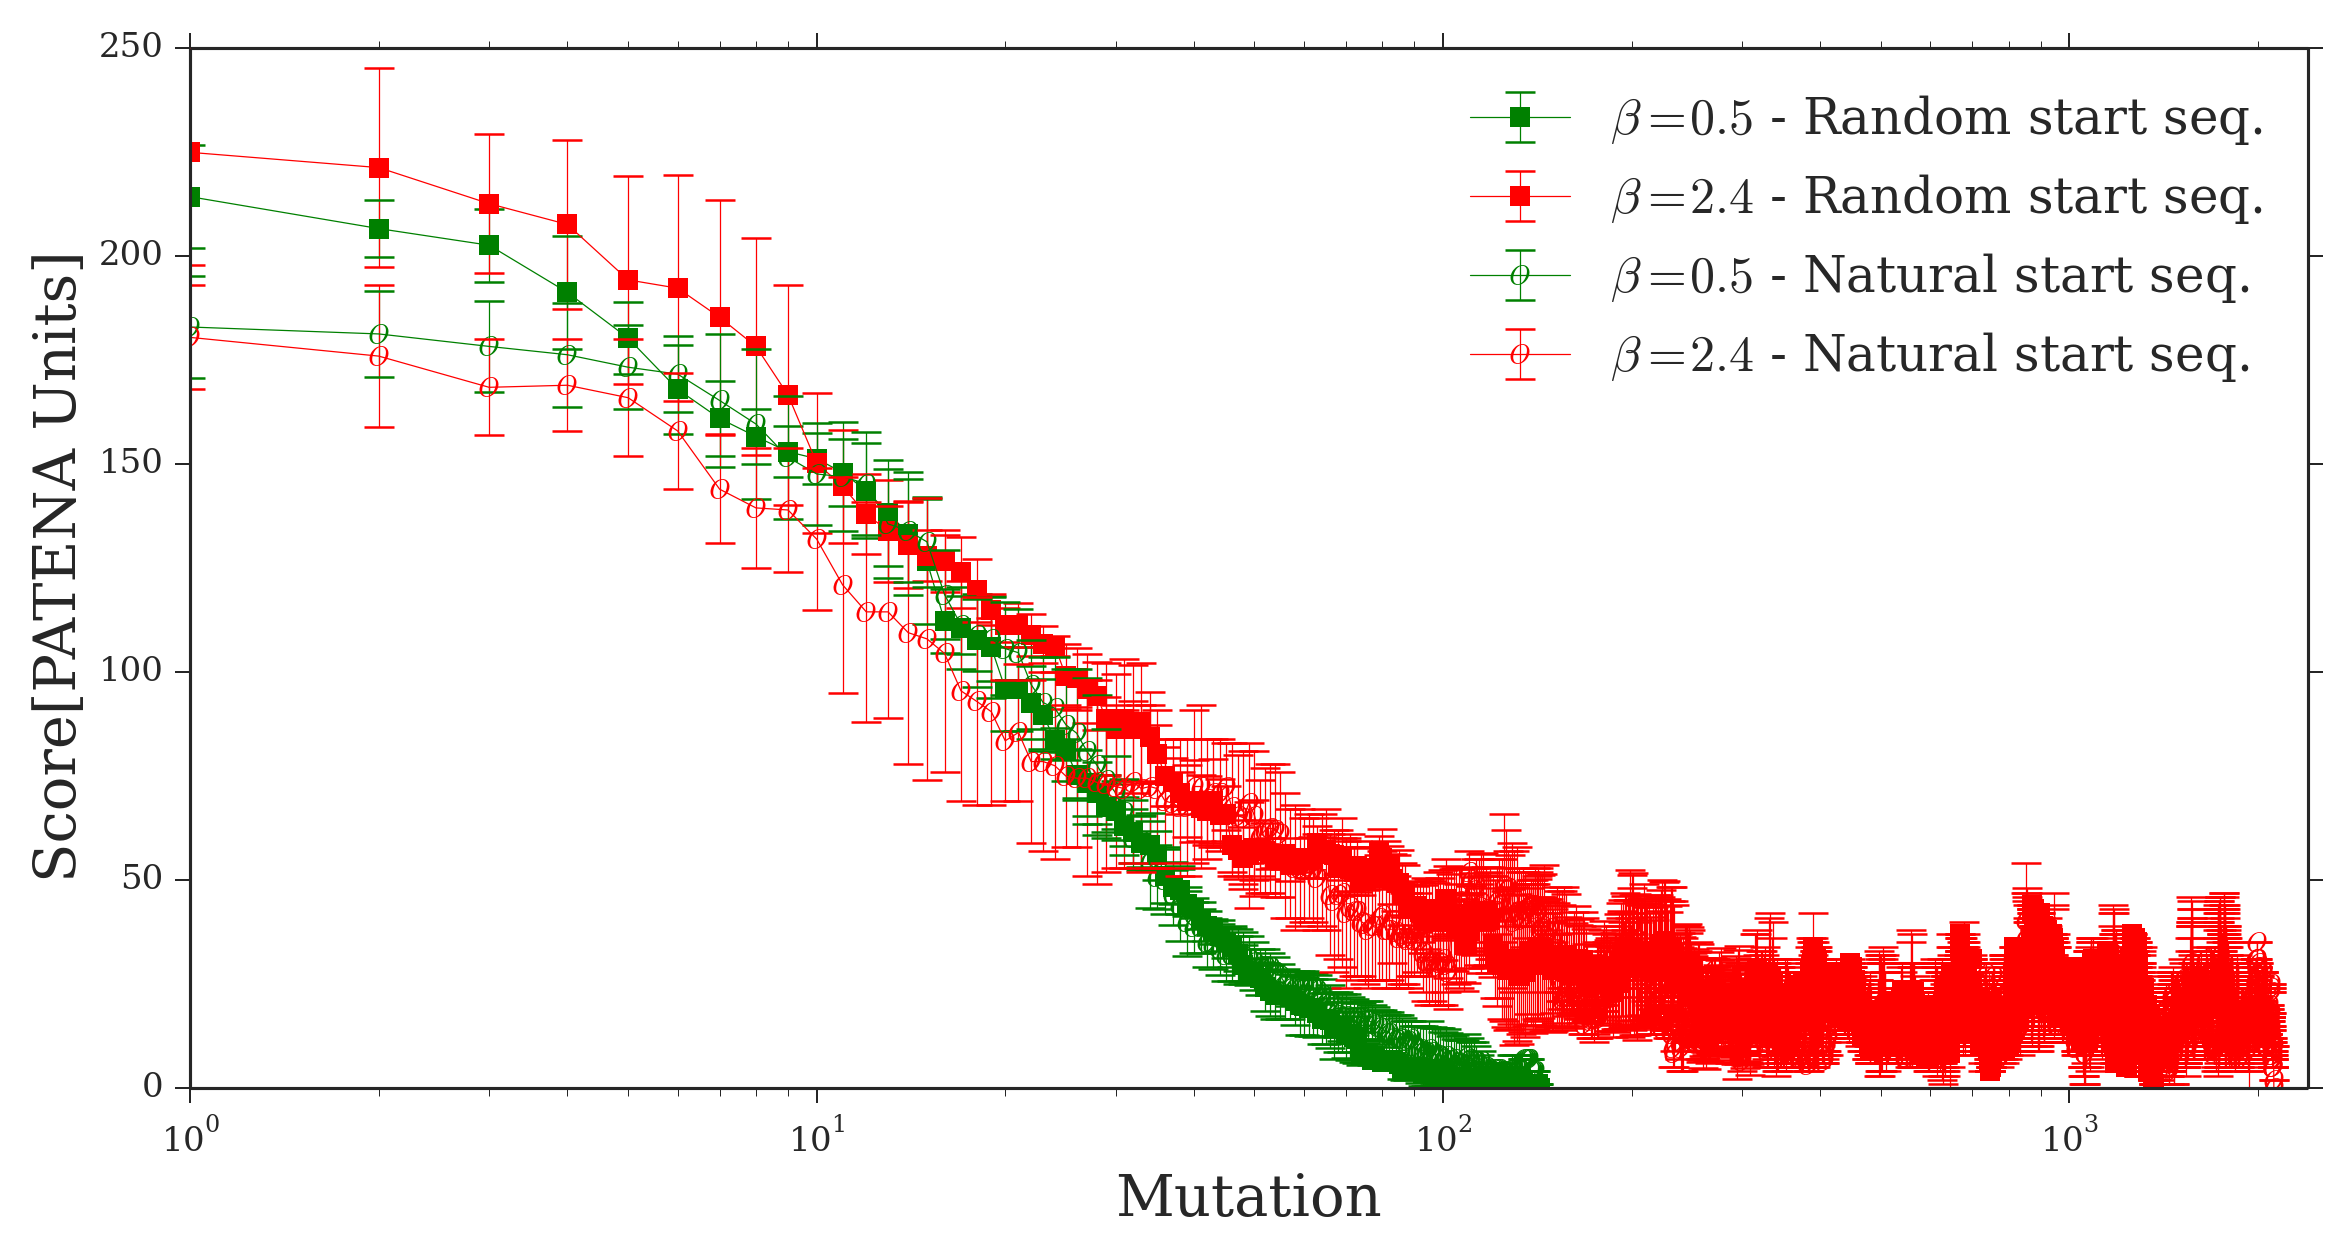
\includegraphics[width=\textwidth]{img/resultados/iterationVsScore-mean.png}
    \caption{Valores medios y desviaciones}
  \label{fig:scoreVsiter-b}
  \end{subfigure}
  \caption{\textbf{Perfil de puntajes asociado a cada iteración para distintos $\beta$}}
  \label{fig:scoreVsiter}
\end{figure}




% \begin{figure} 
% \advance\leftskip-2cm
% \subfigure[Ejecuciones individuales]{\label{fig:mutAttemptsVsite-a}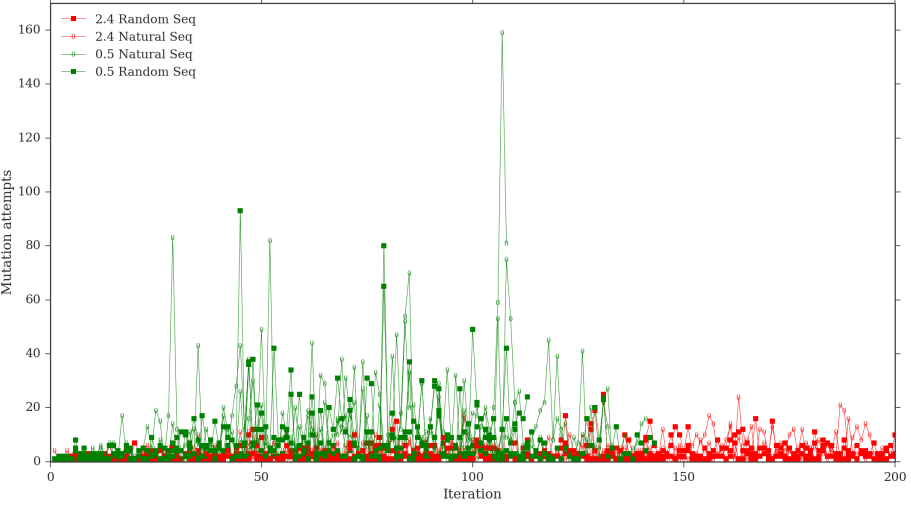
\includegraphics[width=1.15\textwidth]{img/resultados/individuales-mutAt-vs-iter-hasta200.png}}
% \subfigure[Valores medios y desviaciones]{\label{fig:mutAttemptsVsite-b}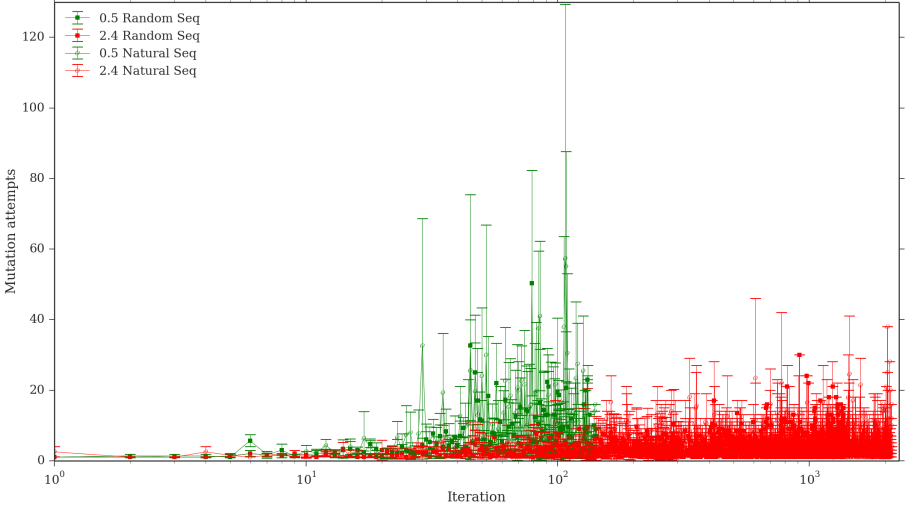
\includegraphics[width=1.15\textwidth]{img/resultados/mutAttemptsVsite-cada1-hasta2270.png}}
% \caption{Dependencia del número de intentos de mutación con la iteración}
% \label{fig:mutAttemptsVsite}
% \end{figure}


% INTENTOS DE MUTACION PARA BETA  0.5 Y 2.4
\begin{figure}[htbp]
% \advance\leftskip-1.5cm
  \begin{subfigure}[b]{\textwidth}
%     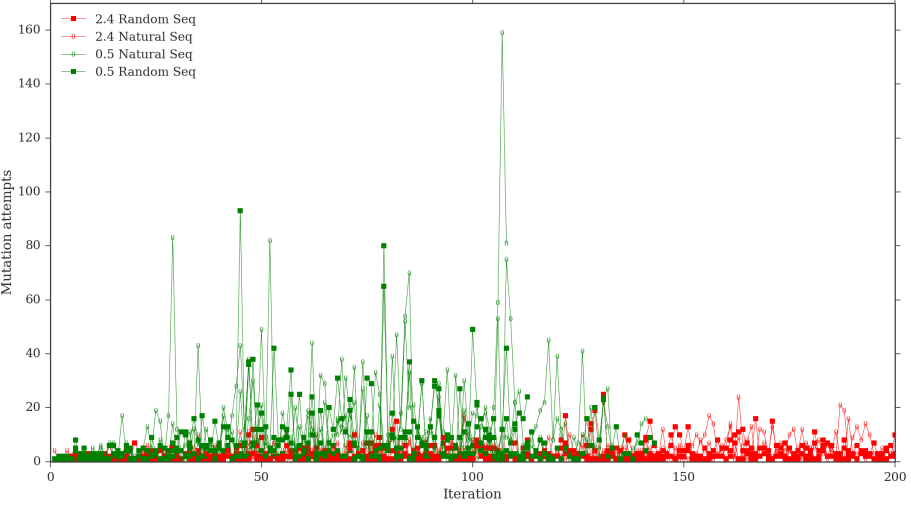
\includegraphics[width=1.15\textwidth]{img/resultados/individuales-mutAt-vs-iter-hasta200.png}
    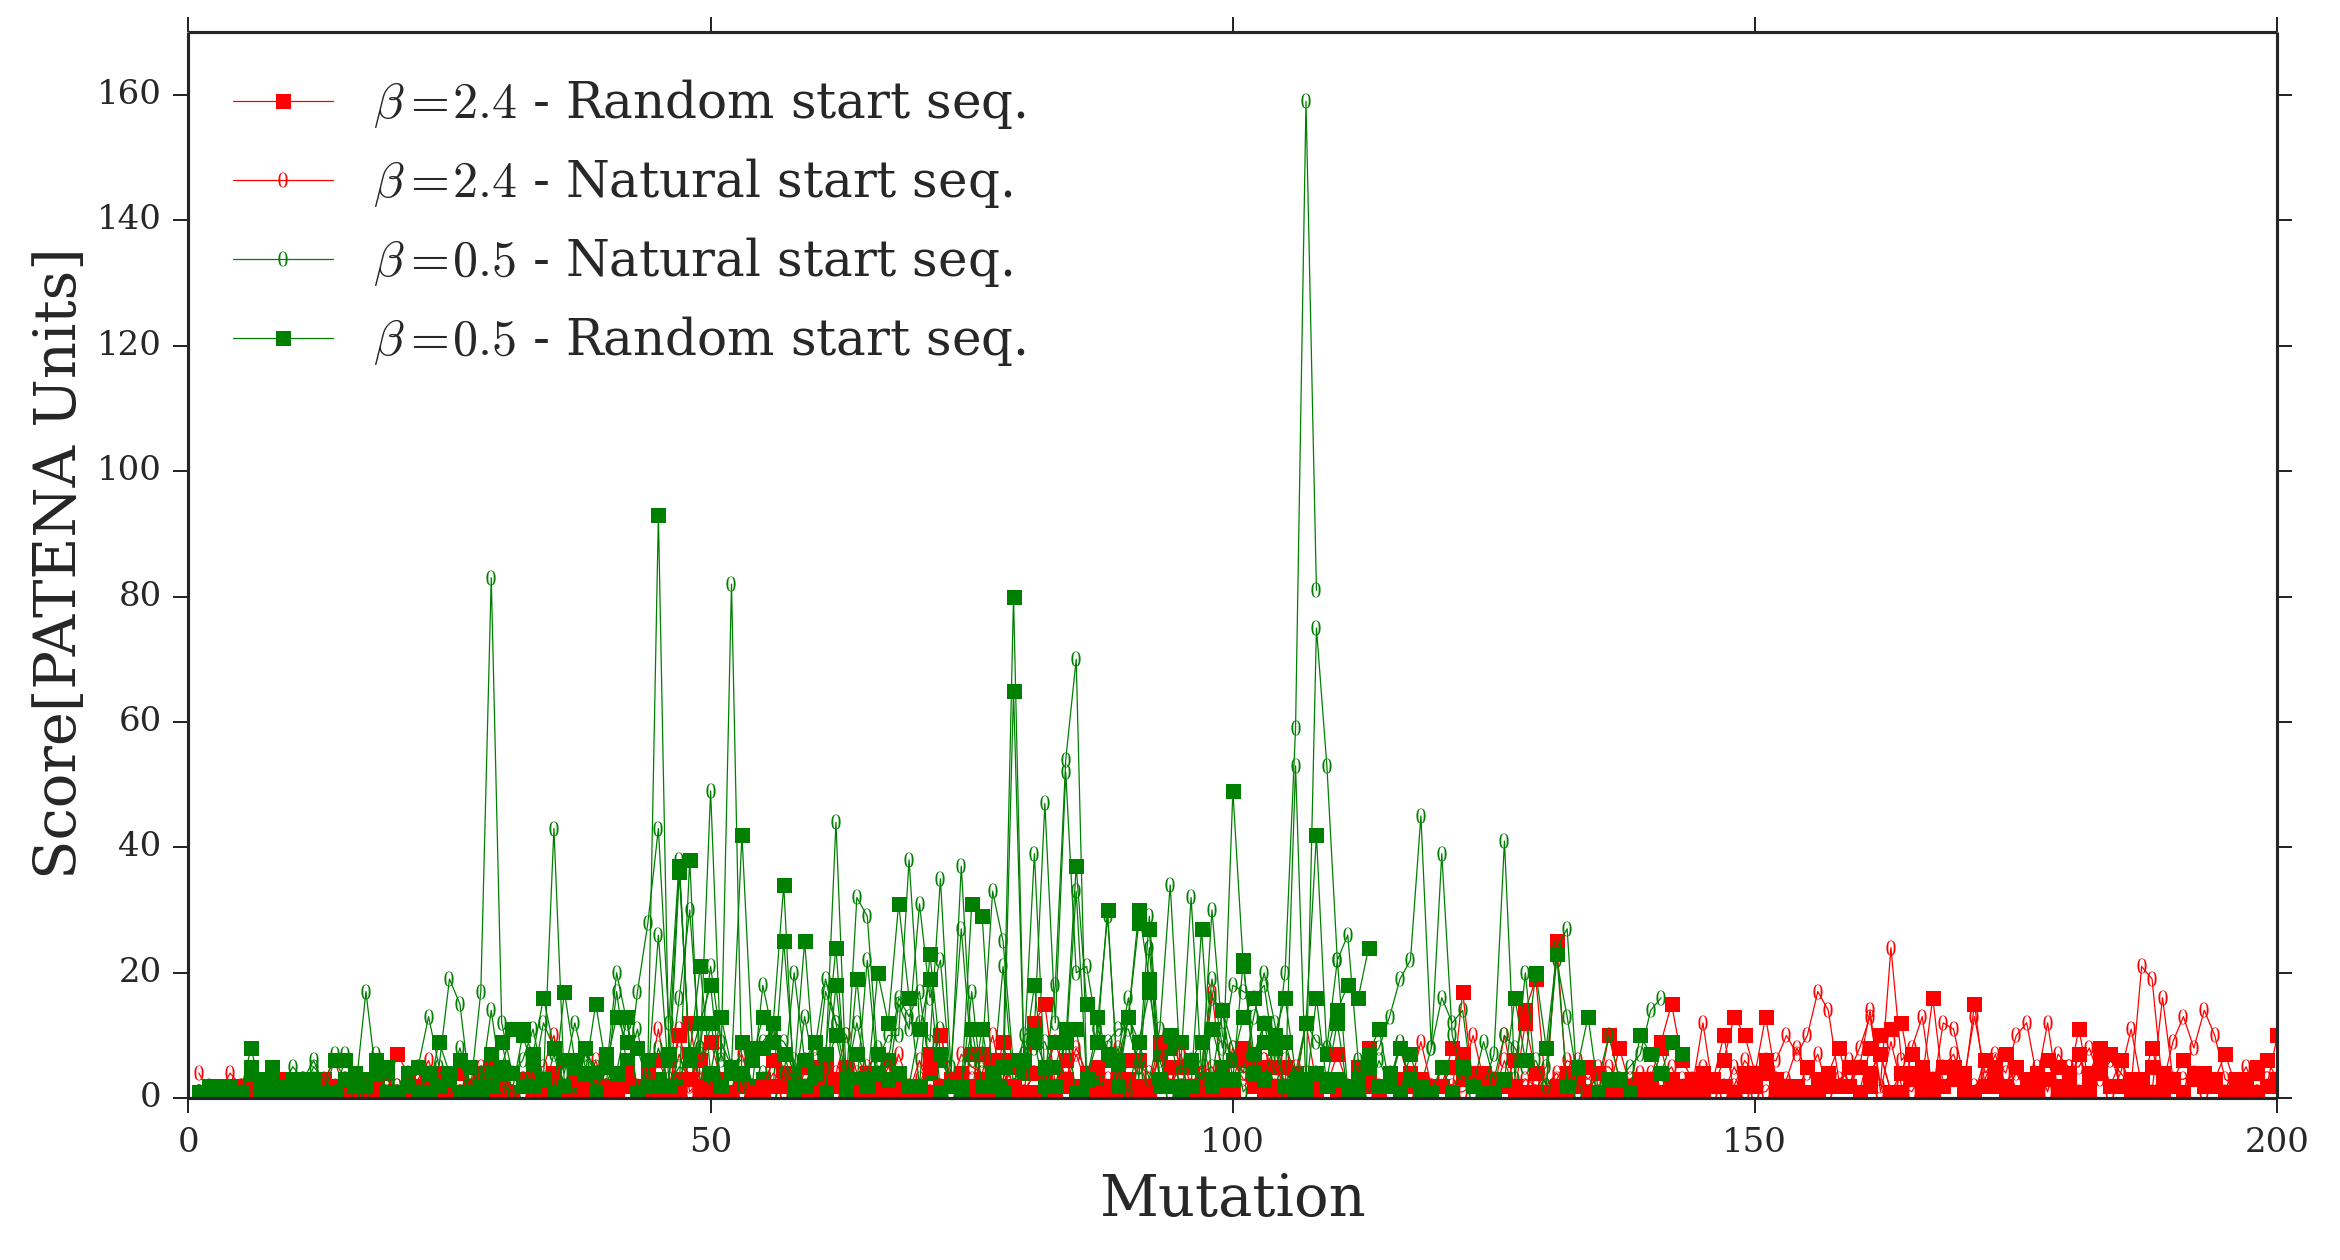
\includegraphics[width=\textwidth]{img/resultados/iterationVsMutAttempts-individual.png}
    \caption{Ejecuciones individuales}
    \label{fig:mutAttemptsVsite-a}
  \end{subfigure}
%   \hspace{20px}
  \begin{subfigure}[b]{\textwidth}
%     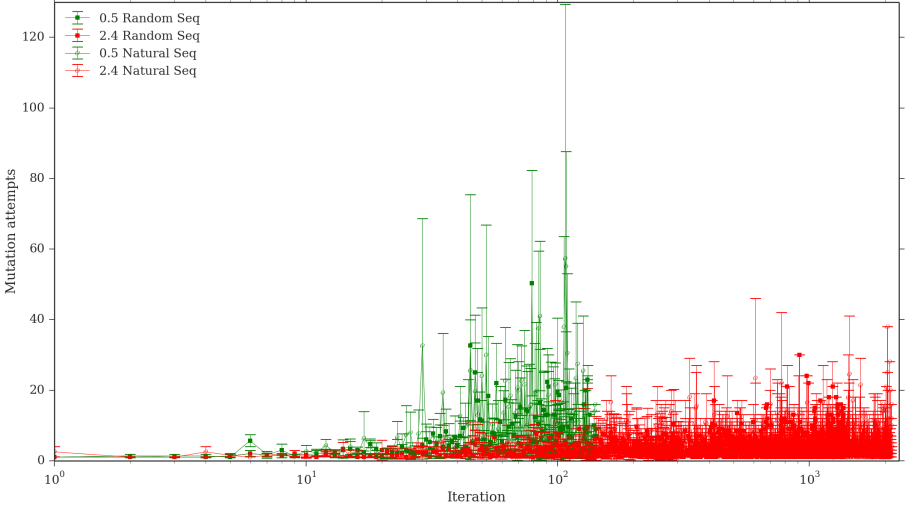
\includegraphics[width=1.15\textwidth]{img/resultados/mutAttemptsVsite-cada1-hasta2270.png}
      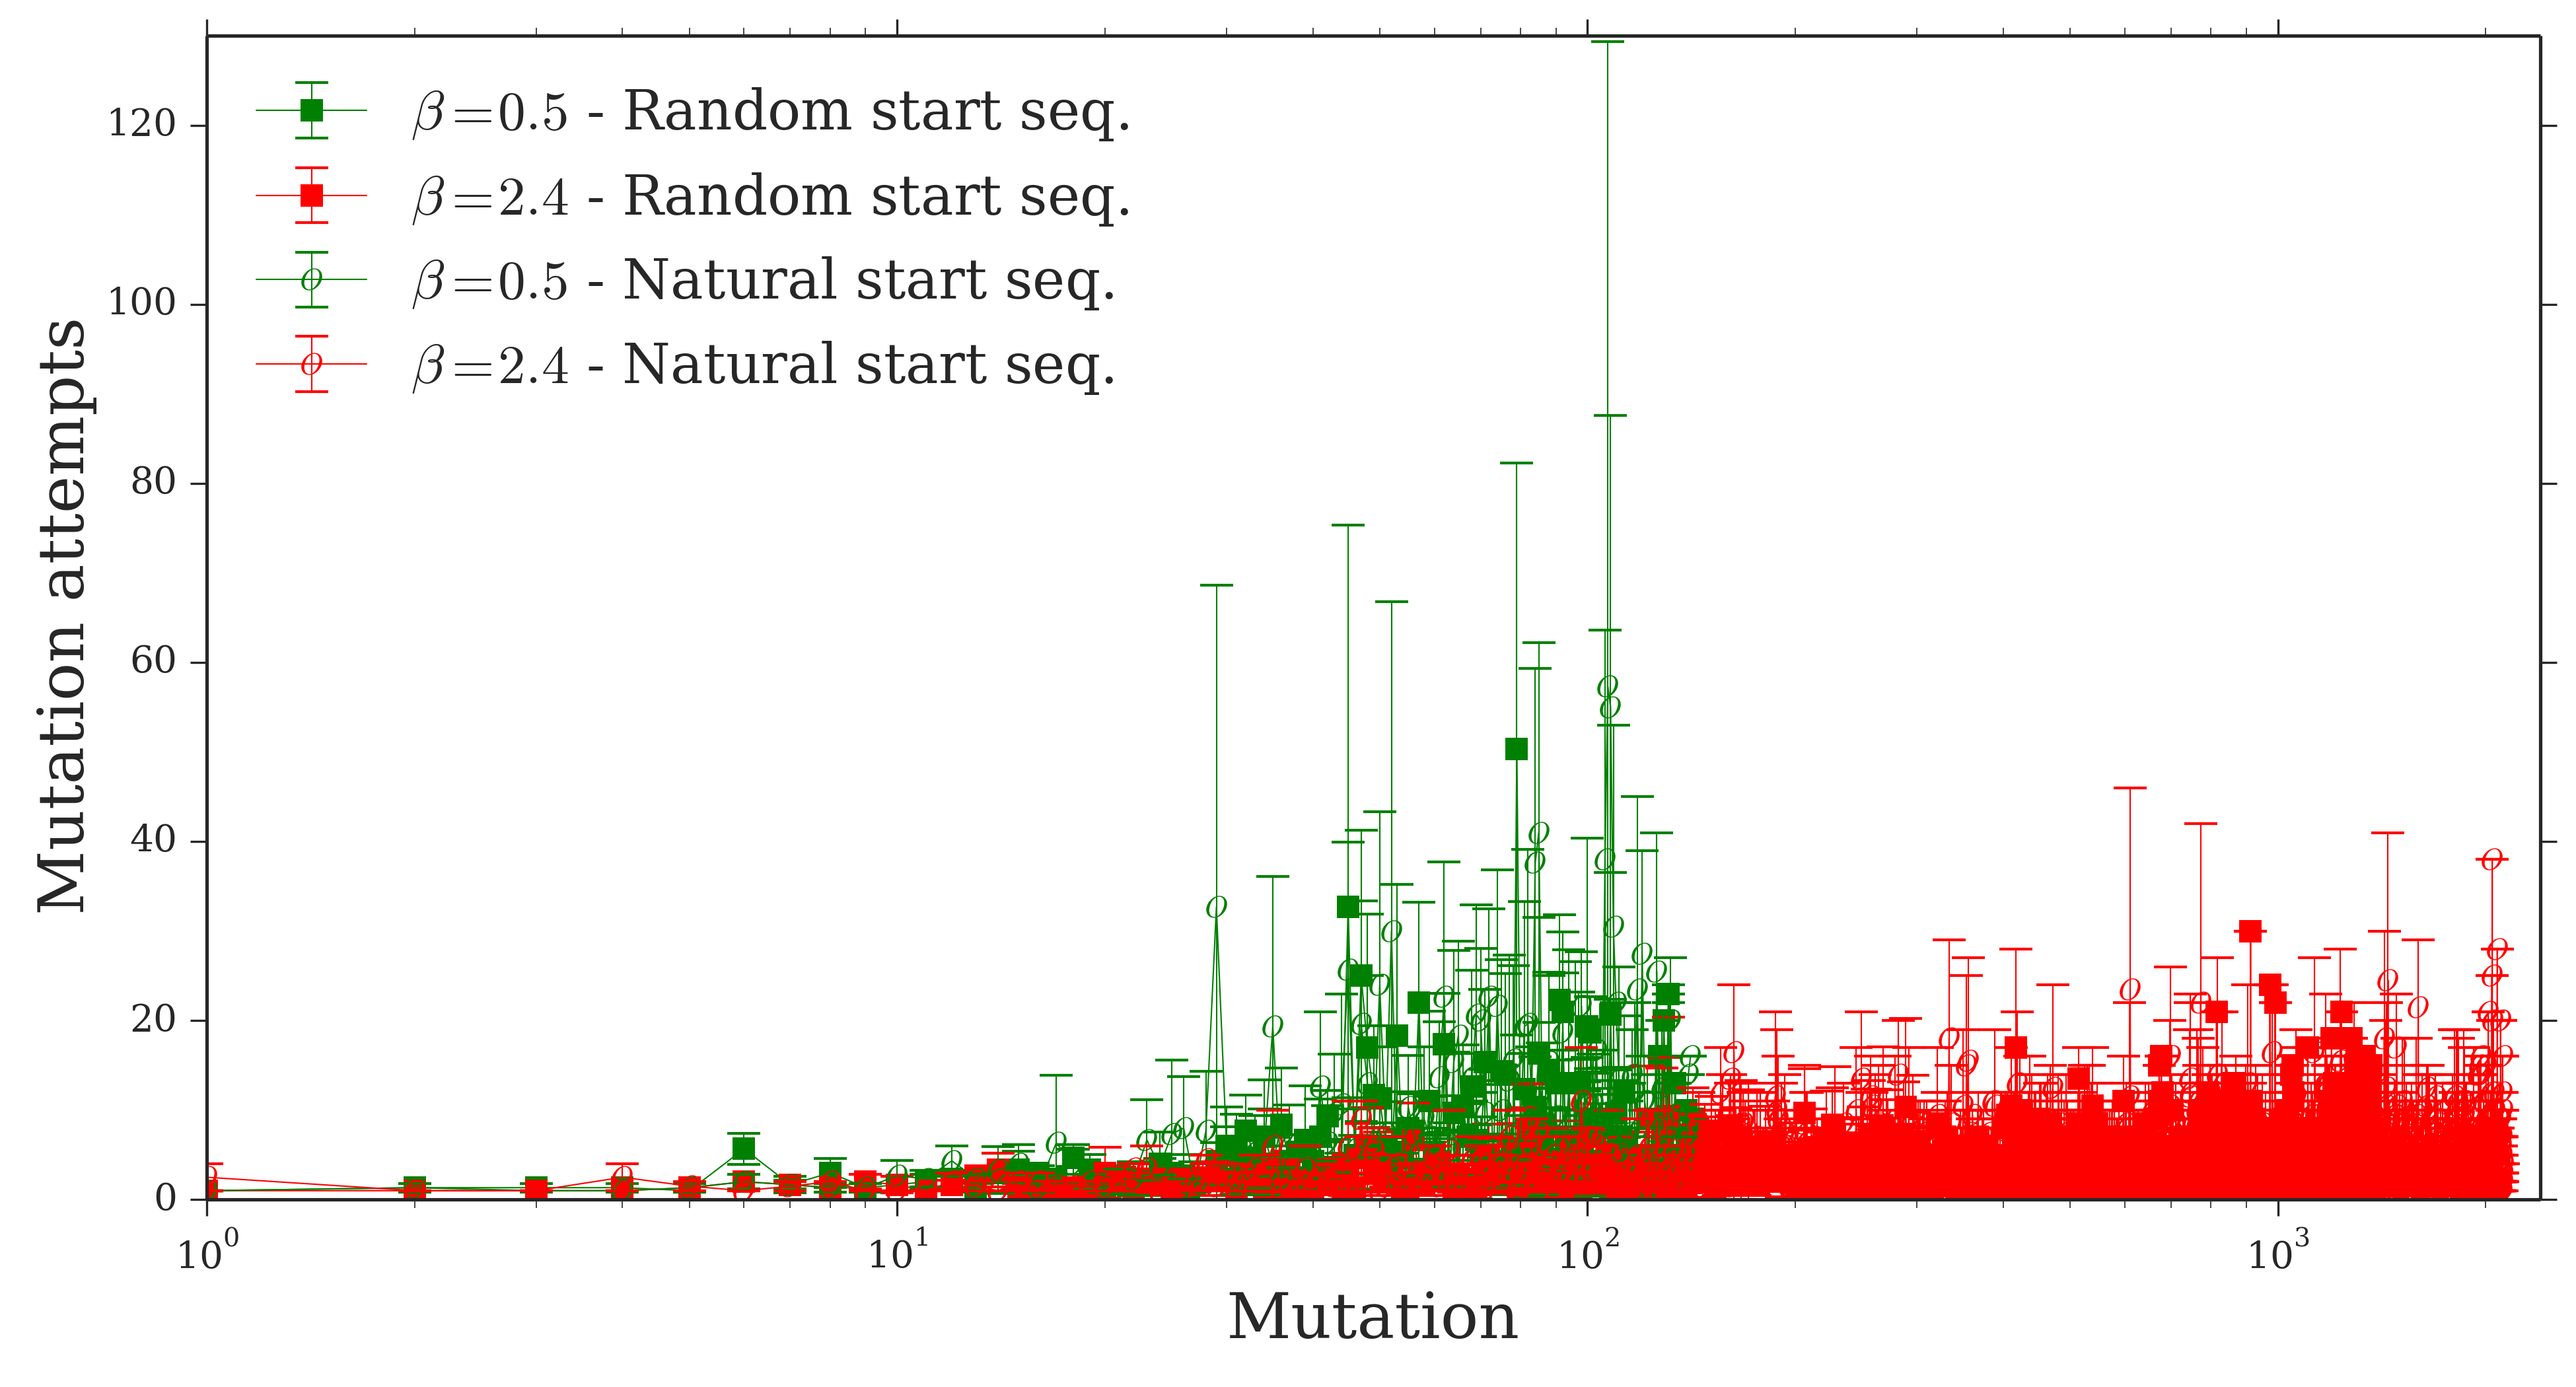
\includegraphics[width=\textwidth]{img/resultados/iterationVsMutAttempts-mean.png}
    \caption{Valores medios y desviaciones}
  \label{fig:mutAttemptsVsite-b}
  \end{subfigure}
  \caption{\textbf{Dependencia del número de intentos de mutación con $\beta$}}
  \label{fig:mutAttemptsVsite}
\end{figure}









% GRAFICO DE SCORE vs ITERACION   (MEDIAS Y StdDeV COMPLETO HASTA EL FINAL)   +  CORRIDAS INDIVIDUALES
En el gráfico \ref{fig:scoreVsiter} se muestra la dependencia del puntaje con las mutaciones aplicadas, tanto los valores medios (y desviaciones estándar) para todas las ejecuciones mencionadas (gráfico \ref{fig:scoreVsiter-b}), 
como el detalle de las ejecuciones individuales (gráfico \ref{fig:scoreVsiter-a}).
El perfil que se muestra permite aclarar mejor los conceptos mencionados previamente acerca de la dependencia de $\beta$ con el comportamiento de la búsqueda. 
Un valor más grande de $\beta$ realiza una mayor exploración del espacio de soluciones, lo que se ve reflejado en un rango mucho más amplio de mutaciones aplicadas para alcanzar el resultado.
Se ve claramente que hay una diferencia en el orden de magnitud de la cantidad de mutaciones aplicadas, donde las ejecuciones con $\beta=$2.4 pueden llegar a alcanzar más de 2000.
Por su parte, el valor más chico de $\beta$ permite alcanzar el objetivo en un número mucho menor de mutaciones, lo cual parece indicar que hay un camino 
que conduce desde cada punto de inicio hacia un resultado bajando continuamente el valor del puntaje, es decir, sin atravesar ninguna barrera.
De todas formas, a partir de este experimento no podemos extraer datos concretos sobre las características de este recorrido hacía el mínimo.
% PONER ALGUNA CONCLUSION DE QUE DICE ESTO ACERCA DE LA SUPERFICIE 

% Esta es, sin embargo, una visión muy general de la ejecución, y para tener una idea mas detallada es necesario analizar otros parámetros relevantes.
% y   MUT-ATTEMPTS vs ITERACION (MEDIAS Y StdDeV COMPLETO HASTA EL FINAL)   +  CORRIDAS INDIVIDUALES
En el gráfico \ref{fig:mutAttemptsVsite} se muestra el número de intentos requeridos para lograr la aceptación de cada mutación aplicada a lo largo de la ejecución.
% asociado a cada valor de $\beta$.
Nuevamente se muestran los valores medios (y sus desviaciones correspondientes) en el gráfico \ref{fig:mutAttemptsVsite-b}, y el detalle de las ejecuciones individuales (gráfico \ref{fig:mutAttemptsVsite-a}).
Vemos que el reducido número de mutaciones necesarias que resulta de un valor bajo de $\beta$ se produce a costa de una cantidad más elevada de intentos previos.
% , previos a aceptar cada mutación. 
Es decir, se evalúa una mayor cantidad de posibles mutaciones hasta que eventualmente una sea aceptada, lo que representa la dificultad del camino hacia el valor mínimo buscado. 
Esta condición se incrementa en las mutaciones cercanas al fin de la ejecución, que se corresponden con los valores más bajos de puntaje (cercanos a 0). 




% basicamente tengo que decir que los tiempos de ejecucion vistos son el resultado del balance entre el numero de intentos de mutacion y el numero de iteraciones totales.

Comprobamos, entonces, que un valor más grande de $\beta$ implica un incremento considerable en el número de mutaciones requeridas, aunque un valor menor de $\beta$ tendrá una mayor cantidad de intentos de mutacion por iteración.
Sabiendo que ambas propiedades impactan negativamente en el proceso de búsqueda incrementando el tiempo de ejecución, 
intentaremos ver ahora cómo, en el rango efectivo de $\beta$, se crea el balance óptimo entre estos parámetros.
% ancean correctamente en el rango efectivo de beta descrito previamente.
% el rango efectivo de beta es producto del balance correcto entre estas propiedades.
% FALTA UNA CONEXION DE LAS EVALUACIONES PREVIAS (PARA BETA 0.5 Y 2.4) CON ESTO NUEVO,  
% Ahora tenemos una idea más clara de cómo afecta beta a los parámetros de exploración. 
% veremos cómo estos parametros se balancean
% intentaremos ver ahora cómo es el balance de estos parámetros con respecto a los distintos valores de beta, para dar los tiempos de ejecución vistos previamente.
% Trataremos de explicar los valores de tiempo de ejecución y el rango efectivo de beta encontrados previamente, basándonos en los parámetros de la búsqueda.
% Es decir, intentaremos explicar cómo la suma entre el número total de mutaciones y de intentos de mutacion producen los tiempos de ejecución encontrados. 
Para esto, analizaremos el perfil completo de las ejecuciones realizadas en la sección previa para encontrar el rango óptimo de $\beta$, 
lo cual se muestra en las figuras \ref{fig:betaVsMut-AttemptsPerit} y \ref{fig:betaVsMutations-Attempts} (no se realiza la separación entre ejecuciones iniciadas a partir de secuencias naturales o secuencias random).

% ACA EMPIEZO A HABLAR DE LOS GRAFICOS DE VALORES  vs RANGO DE BETA:  intentos de mutacion, iteraciones , intentos de mutacion por iteracion
Lo que vemos en la figura \ref{fig:betaVsMut-AttemptsPerit} es que el número de intentos de mutación por iteración baja al aumentar el valor de $\beta$, lo cual es esperable de acuerdo a lo visto previamente.
Sin embargo, según se puede ver en el gráfico \ref{fig:betaVsMutations-Attempts} el número total de intentos de mutación no siempre tiene una disminución correspondiente.
% la disminución no es tan significativa cómo para que disminuya el número de intentos
% Lo que produce esto es que 
En algunas regiones, principalmente para los valores de $\beta$ más altos, el aumento del número de iteraciones es mucho mas significativo que la disminución en los intentos de mutación de cada iteración.
Esto se debe a que, para valores bajos de $\beta$, los intentos de mutación son considerablemente bajos, pero también se debe a que el incremento en el número de iteraciones requeridas es muy alto para valores grandes de $\beta$.
El resultado es que, para valores de $\beta$ superiores a 2.0, el incremento en el número de mutaciones requeridas es tan grande que produce, también, un incremento en el número total de intentos de mutación.
Esto rompe el balance entre ambas propiedades y genera un aumento del tiempo de ejecución, como se vió en la sección anterior.

% De esta forma, 
% Sin embargo, en algunos rangos de beta (entre 0.5 y 1.0, y entre 2.0 y 2.5), no hay una disminución correspondiente del número de intentos totales de mutación al aumentar $\beta$. 
% Según se puede ver en el gráfico \ref{fig:betaVsMutations-Attempts}, el gran número de mutaciones totales requeridas genera un incremento en el número total de intentos de mutación. 

% De esta forma, para valores muy grandes de beta no se logran un balance de 
% Sin embargo, el número de mutaciones totales de la ejecución no siempre disminuye junto con $\beta$. 
% En algunos rangos de $\beta$ (como por ejemplo entre 0.1 y 0.5 , y entre 1.0 y 2.0), 
% En el extremo inferior ($\beta$ <= 0.5), el número total de mutaciones disminuye con $\beta$, mientras que el en rango de 










% BETA vs ITERACIONES y MUTACIONES TOTALES
% BETA vs INTENTOS DE MUTACION 
\begin{figure}[htbp]
% \advance\leftskip-1.5cm
  \begin{subfigure}[b]{0.9\textwidth}
%     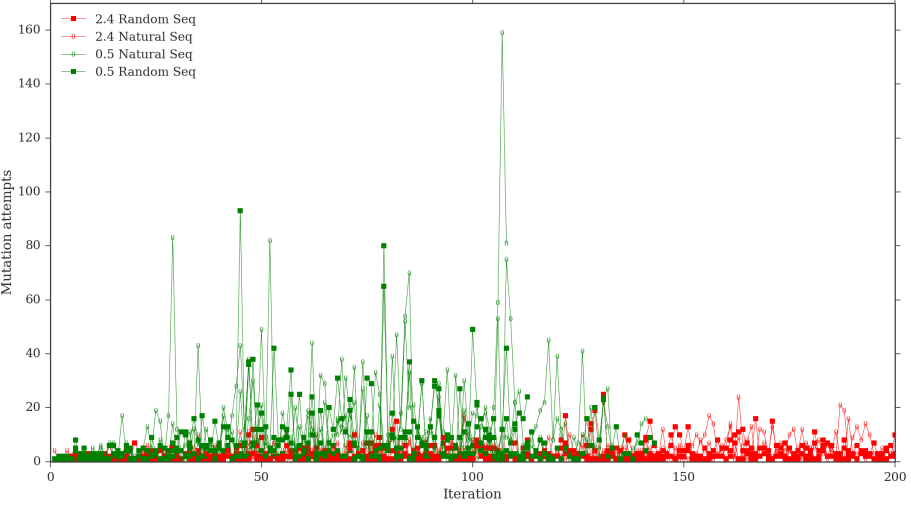
\includegraphics[width=1.15\textwidth]{img/resultados/individuales-mutAt-vs-iter-hasta200.png}
    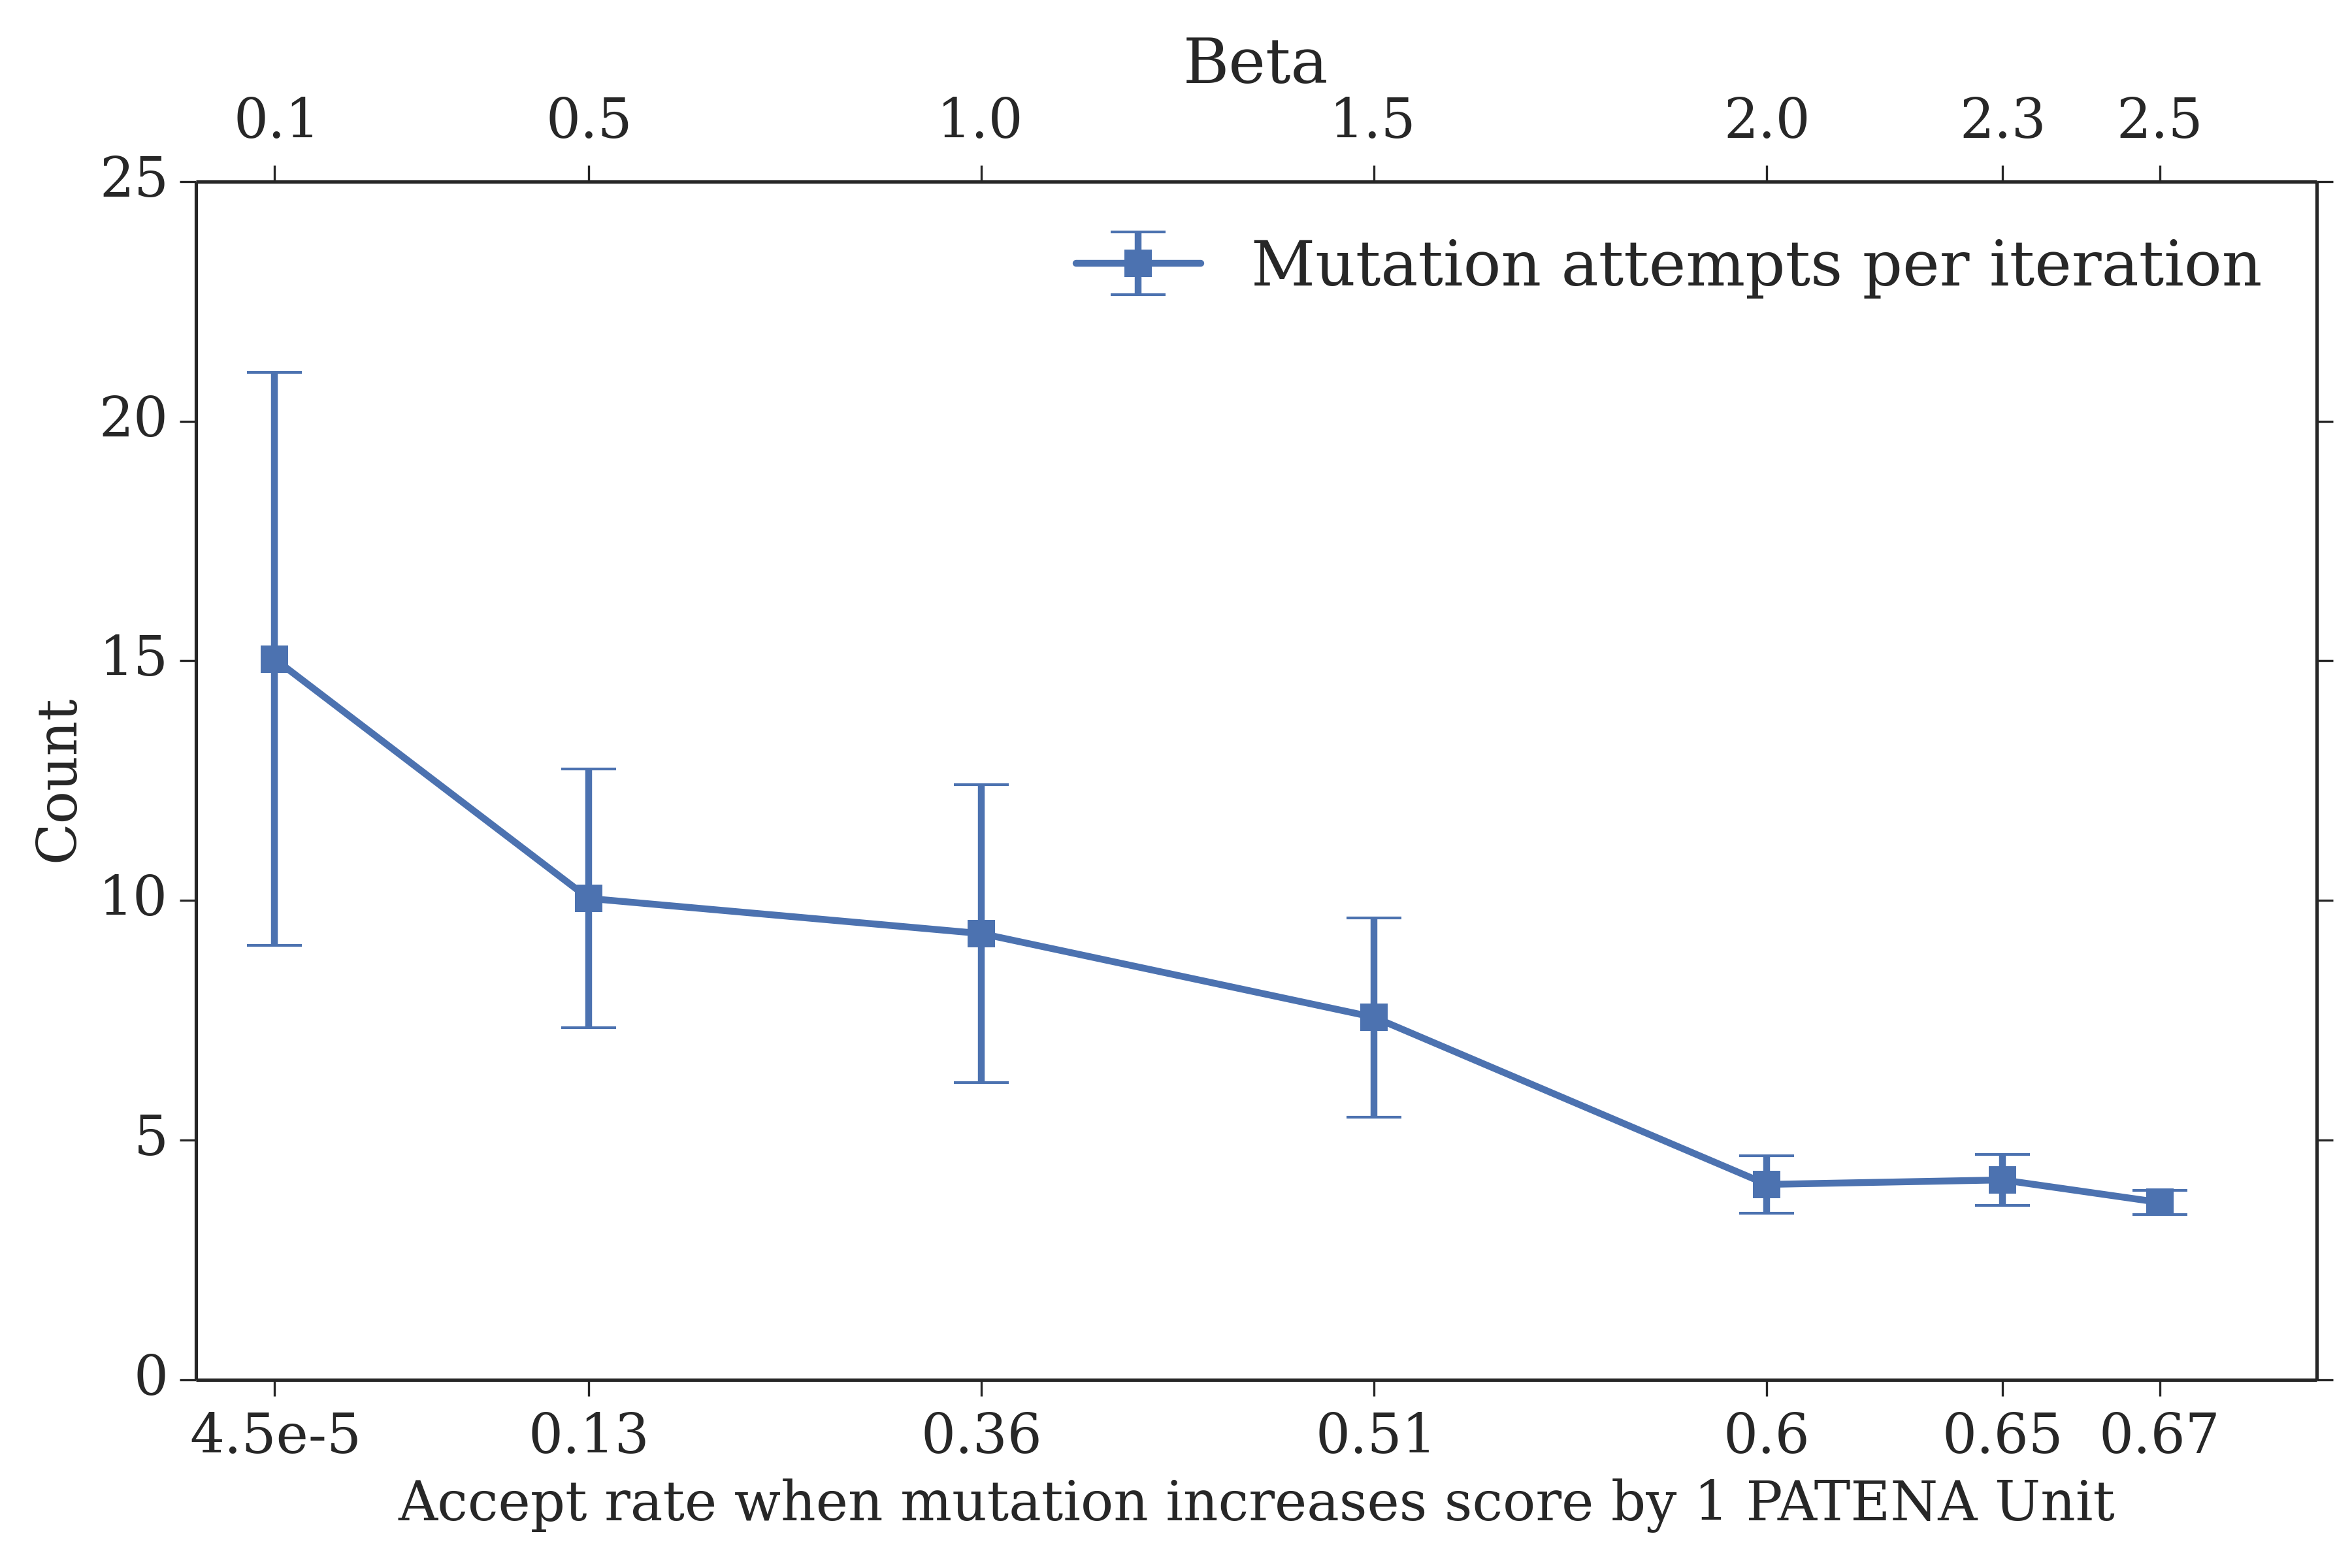
\includegraphics[width=\textwidth]{img/resultados/beta-vs-Mut-iterationsPerIt.png}
    \caption{}
%     LOS INTENTOS DE MUTACION DISMINUYEN CASI SIEMPRE CON EL AUMENTO DE BETA
    \label{fig:betaVsMut-AttemptsPerit}
  \end{subfigure}
%   \hspace{20px}
  \begin{subfigure}[b]{0.9\textwidth}
%     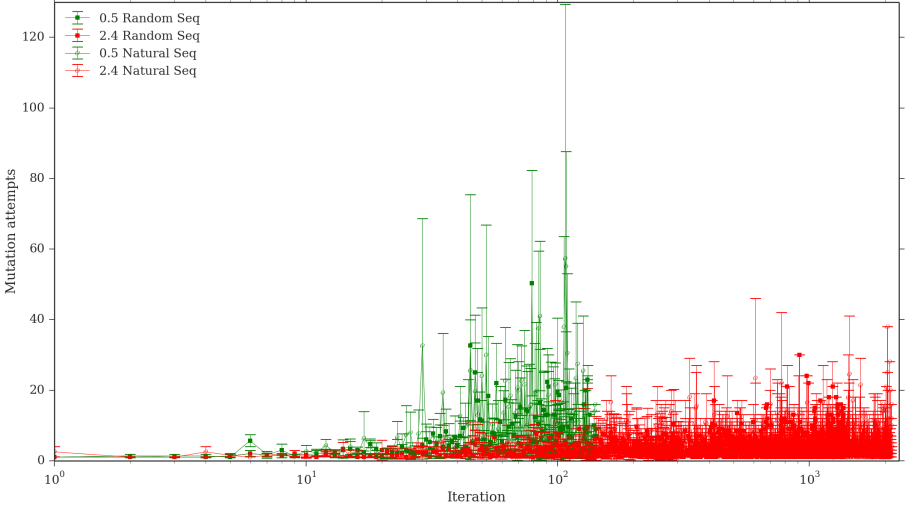
\includegraphics[width=1.15\textwidth]{img/resultados/mutAttemptsVsite-cada1-hasta2270.png}
      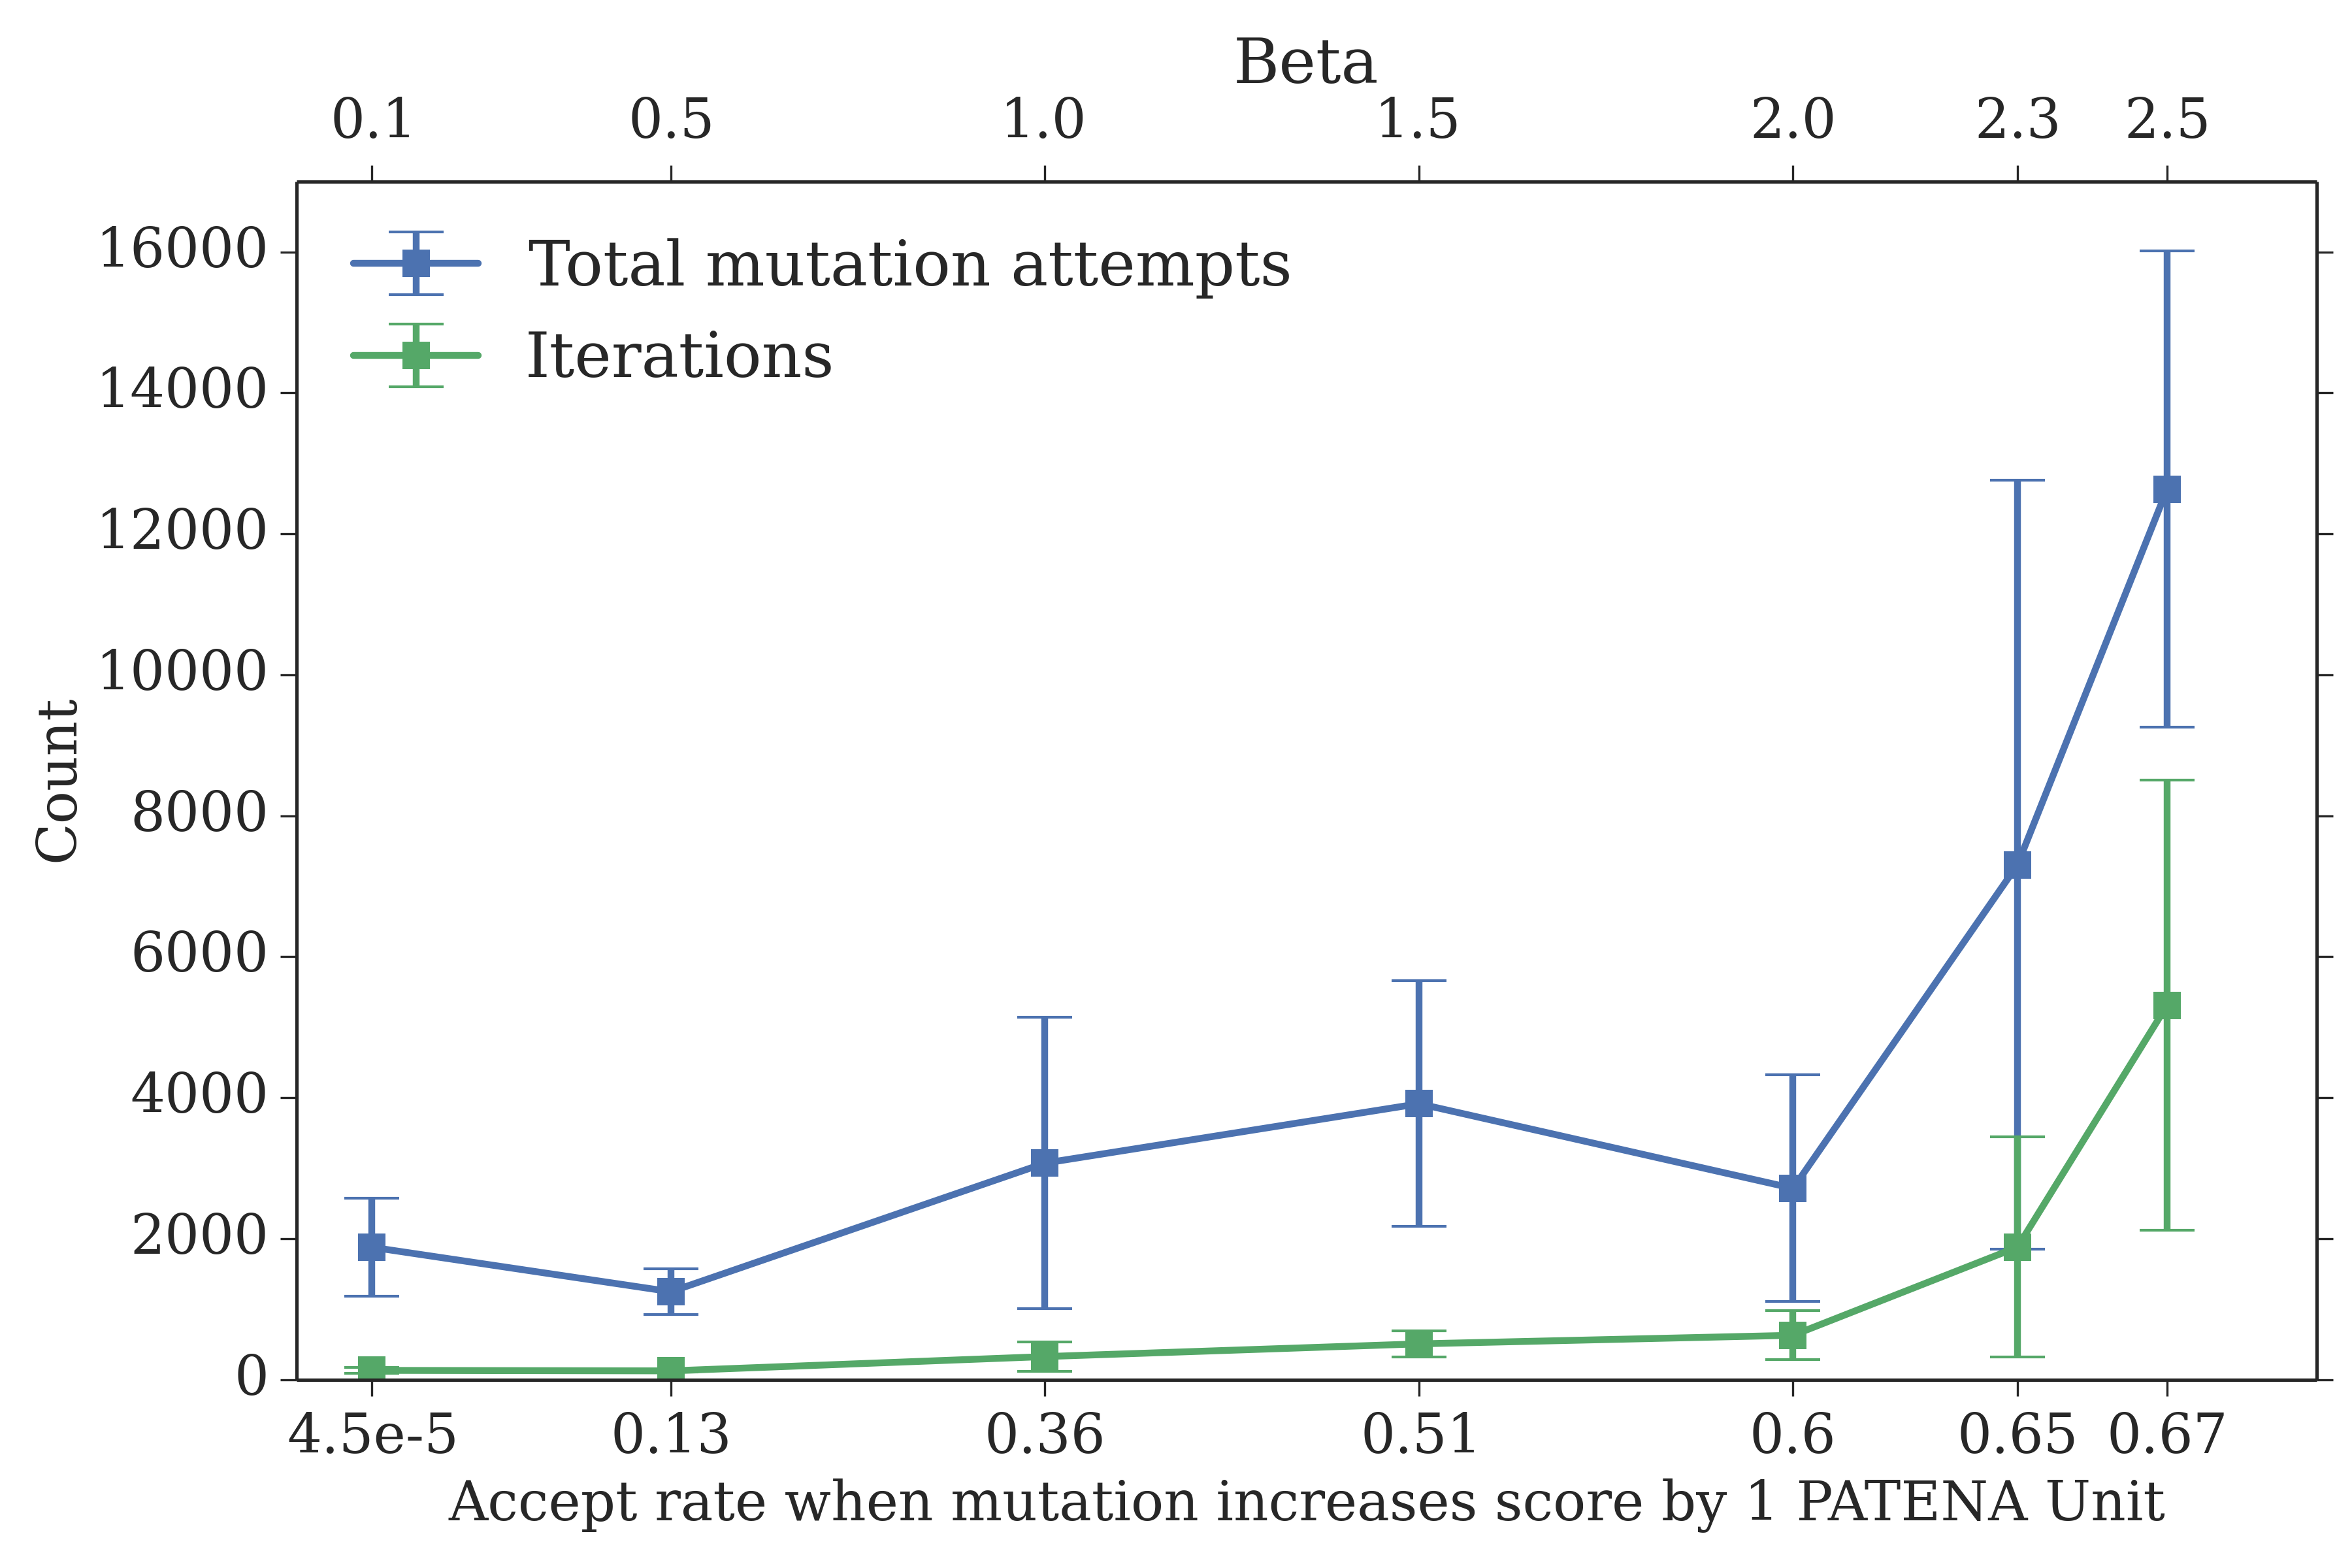
\includegraphics[width=\textwidth]{img/resultados/beta-vs-Mut-iterations.png}
    \caption{}
  \label{fig:betaVsMutations-Attempts}
  \end{subfigure}
  \caption{\textbf{Dependencia de los parámetros de la búsqueda con el valor de beta}}
  \label{fig:betaVsAll}
\end{figure}











\section{Dependencia con la longitud de la secuencia}

% RESULTANDOS DE TIEMPO EN FUNCION DE LONGITUD
Una vez definido un valor de $\beta$ que permite un balance estable entre intentos de mutación y mutaciones aceptadas, queremos saber cómo se traduce esto en un tiempo de ejecución concreto para distintos casos de uso de la herramienta.
Se realizan, entonces, evaluaciones del tiempo de ejecución en función de la longitud de la secuencia, lo que nos dará una idea del orden de tiempo que demoran las ejecuciones y como éste varía con la longitud.
% Utilizando los parámetros estándar, el tiempo de ejecución solo varía con la longitud de la secuencia. 
En el gráfico \ref{fig:time-vs-length} se muestran los resultados de distintas ejecuciones individuales de la aplicación, utilizando siempre el valor de $\beta$ definido previamente (1.0) pero con longitudes de secuencia variable, 
tanto para secuencias aleatorias como para secuencias iniciales naturales.

Si bien los resultados parecen indicar una relación aproximadamente lineal entre la longitud de la secuencia y el tiempo de ejecución, la relevancia de estos resultados es que nos permiten 
saber que la solución es aplicable a secuencias en el rango esperado de utilización de la herramienta. 

\begin{figure}[htbp]
\centering
% 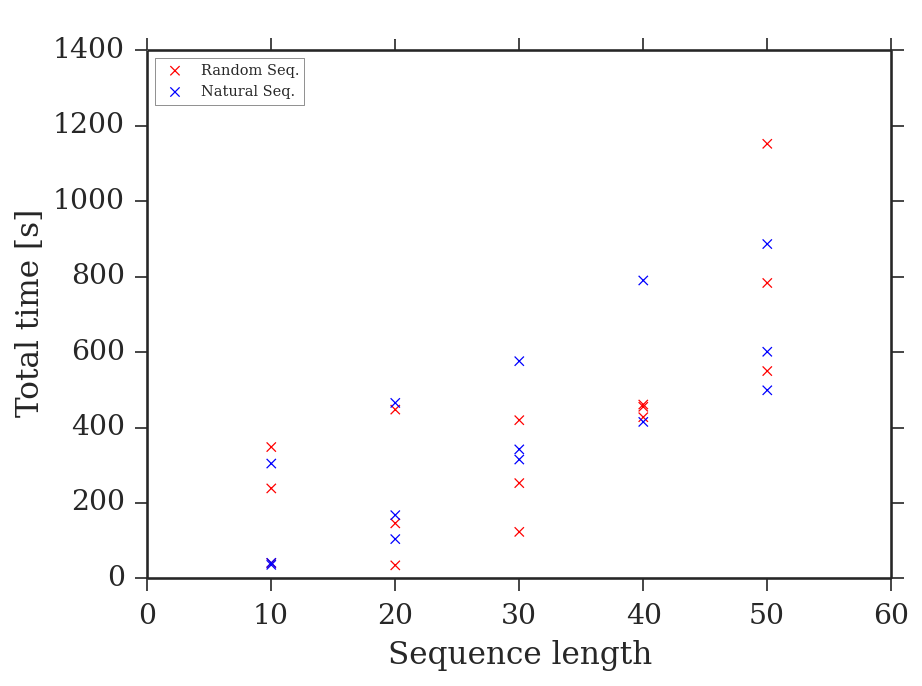
\includegraphics[width=0.8\textwidth]{img/resultados/time-vs-length-beta1.png}
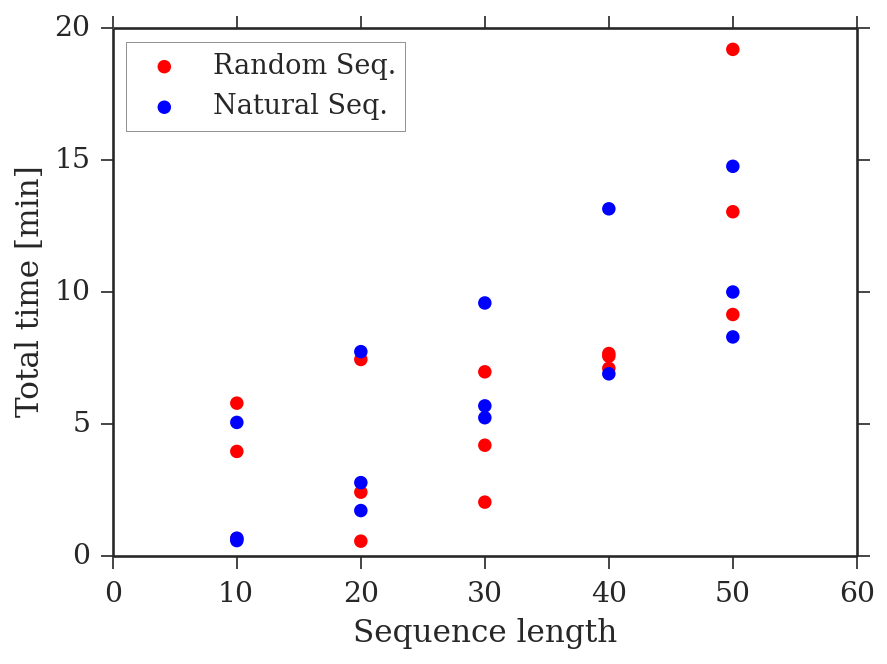
\includegraphics[width=0.7\textwidth]{img/resultados/lengthVsTime.png}
\caption{\textbf{Dependencia del tiempo de ejecución con la longitud de la secuencia}}
\label{fig:time-vs-length}
\end{figure}





\section{Análisis de diseños resultantes}

% DIVERGENCIA EN EL CONJUNTO DE RESULTADOS
Ahora que tenemos fijados todos los aspectos de ejecución del método y que efectivamente podemos obtener, en un tiempo aceptable, secuencias que cumplen con requerimientos definidos, nos centraremos en 
conocer más acerca de los diseños resultantes.


% En primer lugar se analizaron los porcentajes de mutación para cada posición de la secuencia, los cuales se muestran en la figura \ref{fig:mutationPerSite}.
% Si bien no hay ninguna diferencia significativa en el patrón de mutaciones, las 4 posiciones que presentan el menor porcentaje medio de mutaciones (residuos 9,18,19,21),
% se corresponden con residuos de Prolina y Glicina.
% \begin{figure}[h]
% 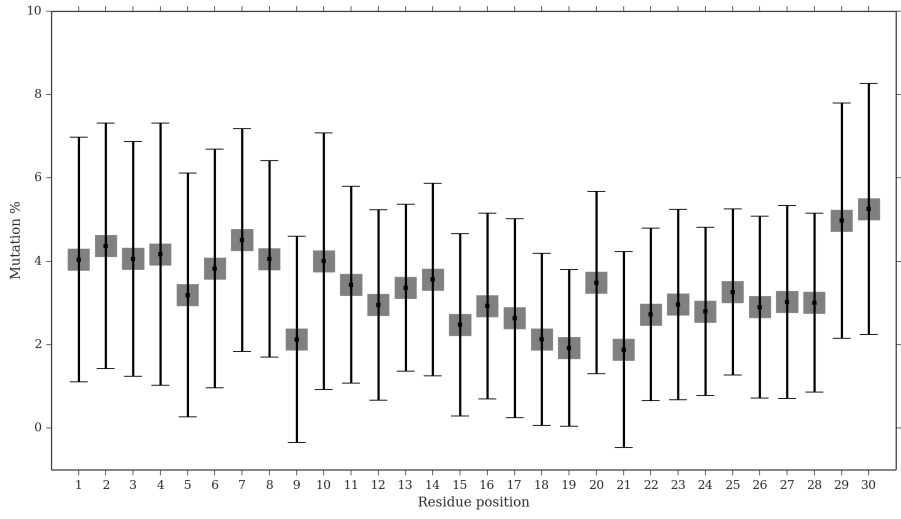
\includegraphics[width=\textwidth]{img/resultados/mutationsPerPosition.png}
% \caption{Procentaje de mutaciones medio para cada posición en 74 corridas individuales}
% \label{fig:mutationPerSite}
% \end{figure}

% ANALISIS DE LA IDENTIDAD SECUENCIAL
Por definición del método, sabemos que los resultados tendrán las propiedades positivas buscadas y no tendrán las características negativas pero, hasta el momento, no sabemos nada más acerca de los diseños que se pueden obtener.
Para comenzar a analizar los diseños resultantes se realizaron un total de 74 ejecuciones independientes a partir de una misma secuencia inicial de largo=30 (\texttt{MALWMRLLPLLALLALWGPDPAAAFVNQHL}).
% INDICAR COMO SE GENERAN LAS SECUNCIAS RANDOM PARA COMPARAR
De forma independiente, mediante la herramienta RandSeq \cite{randseq}, se obtuvieron 1000 secuencias al azar de largo=30 utilizando la composición estándar de nuestro método.
Este \textit{background} representa la máxima diversidad secuencial alcanzable con esta composición.
% para poder analizar estos resultados de forma comaprativa, se generan un background de XX secuencias random, generadas utilizando la herramienta RandSeq \cite{randseq}, utilizando la composición estándar de nuestro método.
% representa la maxima diversidad alcanzable con la composición standard.
% En la figura \ref{fig:identity} se muestran distintas evaluaciones de identidad que involucran a la secuencia inicial y las secuencias de estos conjuntos  
Dado que todas las secuencias random, resultantes e incial tienen la misma longitud, las evaluaciones de identidad entre estas secuencias (mostradas en la figura \ref{fig:identity}) 
se realizaron a partir del número de residuos idénticos encontrados en posiciones correspondientes del par de secuencias. 
El porcentaje de identidad resultante se calcula como: 
\begin{equation}
 \large \bigg(\frac{\text{Número de posiciones con residuos idénticos}}{\text{Largo de la secuencia}}\bigg)*100
\end{equation}

\vspace{0.3cm}

% 
% 
% En primer lugar se analizaron las características secuenciales del conjunto de resultados obtenidos, evaluando el procentaje de identidad secuencial entre estos y con la secuencia inicial. 
Como se ve en la figura \ref{fig:identity} (izquierda), los diseños obtenidos a partir de este ensayo, a pesar de tener una similitud mayor que la encontrada entre secuencias random, se 
muestran como un conjunto considerablemente heterogéneo. Esto confirma que el método permite obtener la diversidad buscada en los diseños resultantes a partir del uso de la composición estándar.
% no poseen una similitud considerable entre sí. 
% EXPLICACION DE LA DIVERSIDAD RESULTANTE
% Esta heterogeneoidad del conjunto de resultados puede explicarse......
% Teniendo en cuenta los fundamentos del método, que describen a las secuencias buscadas como un conjunto amplio y complejo, y las características no determinísticas del método,
% es posible pensar que debería existir al menos cierta diversidad entre los resultados, aún cuando se comparen los resultados de ejecuciones que comienzan en una misma secuencia inicial.
% Hasta el momento vimos el proceso de ejecución analizando de forma abstracta el número de iteraciones, sin tener en cuenta sobre que posiciones se aplicaban,
% sin embargo, la diversidad resultante de la búsqueda dependerá fuertemente del número y distribución de mutaciones que se aplican sobre la secuencia inicial.
% EXPLICACIÓN DE LA SIMILITUD CON LA SECUENCIA INICIAL
Por otro lado, en la figura \ref{fig:identity} (derecha) se muestra que el conjunto de resultados, en comparación con el conjunto de secuencias random, tiene un porcentaje mayor de similitud con la secuencia inicial. 
De esta forma, aún habiendo una gran cantidad de mutaciones, los diseños obtenidos conservan cierta similitud con la secuencia inicial propuesta. 
Esta similitud remanente comprende una ventaja del método ya que permite al usuario proponer un diseño y obtener resultados que presentan cierta similitud con este.
% El conjunto de resultados obtenidos
% que es considerablemente mayor al encontrado cuando se compara un conjunto de secuencias random.
% % \advance\leftskip-2cm
% \centering
% \subfigure[h][Identidad entre las secuencias resultantes(74) y la secuencia inicial]{\label{fig:identity-a}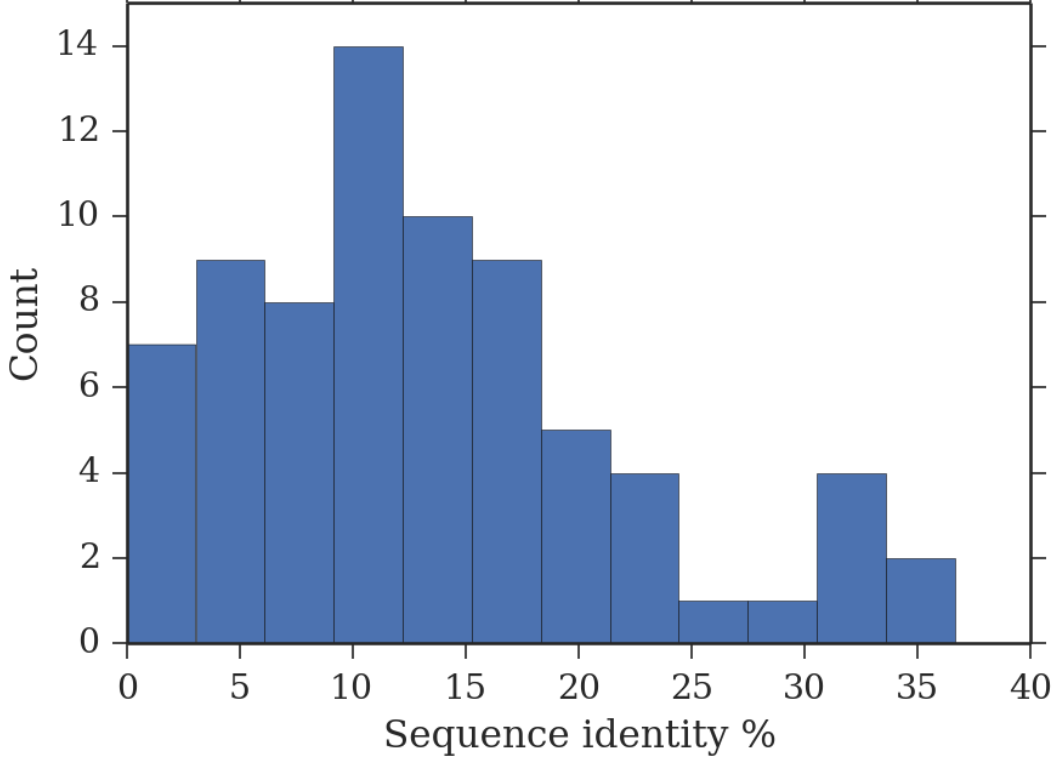
\includegraphics[width=0.5\textwidth]{img/resultados/againstStartSeq-74.png}}
% \subfigure[h][Identidad entre cada par posible de secuencias resultantes(74*74)]{\label{fig:identity-b}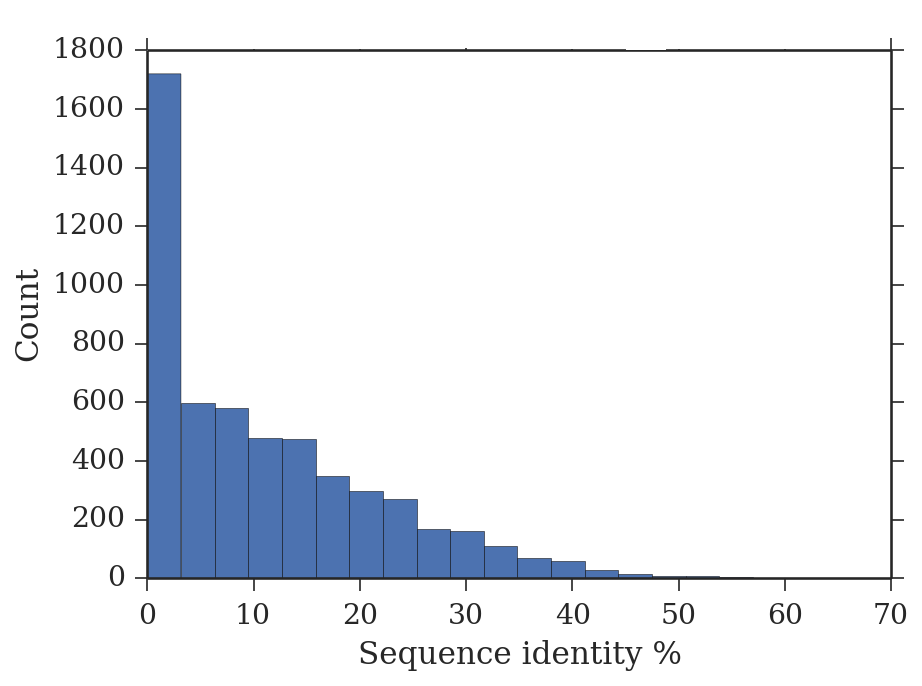
\includegraphics[width=0.5\textwidth]{img/resultados/againstAll-74-borrado.png}}
% \caption{Histograma de identidad de las secuencias resultantes}
% \label{fig:identity}
% \end{figure}



\begin{figure}[htbp]
% \advance\leftskip-1.2cm
  \begin{subfigure}[b]{200px}
%     \caption{}
%     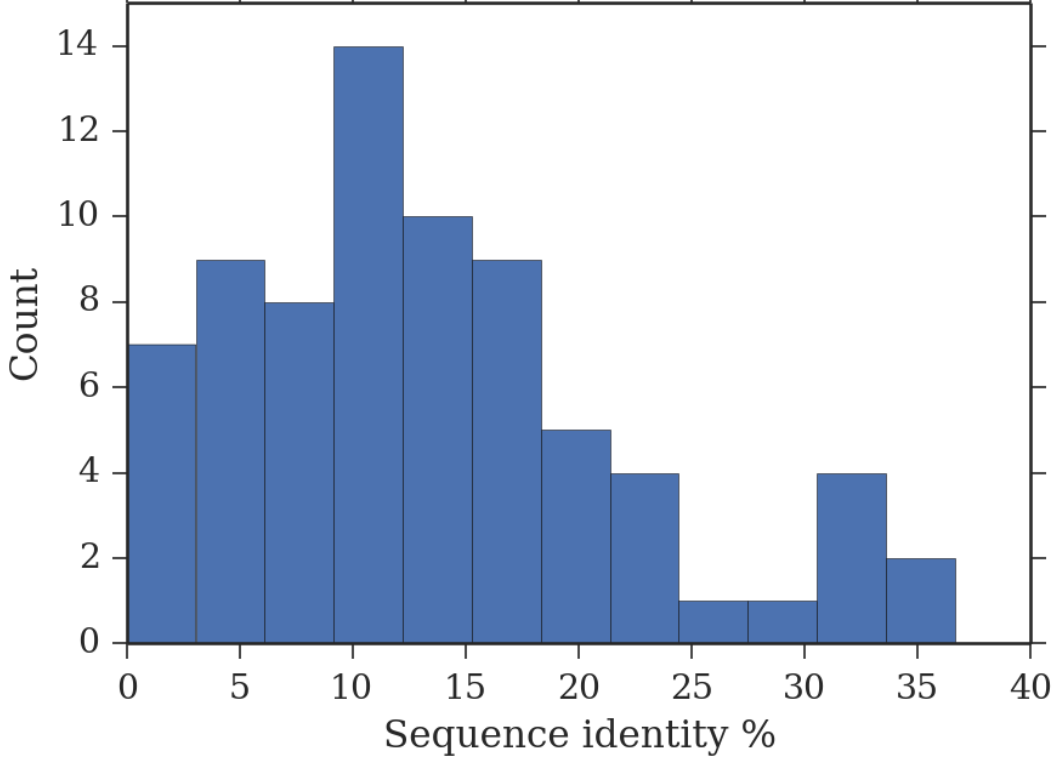
\includegraphics[width=240px]{img/resultados/againstStartSeq-74.png}
    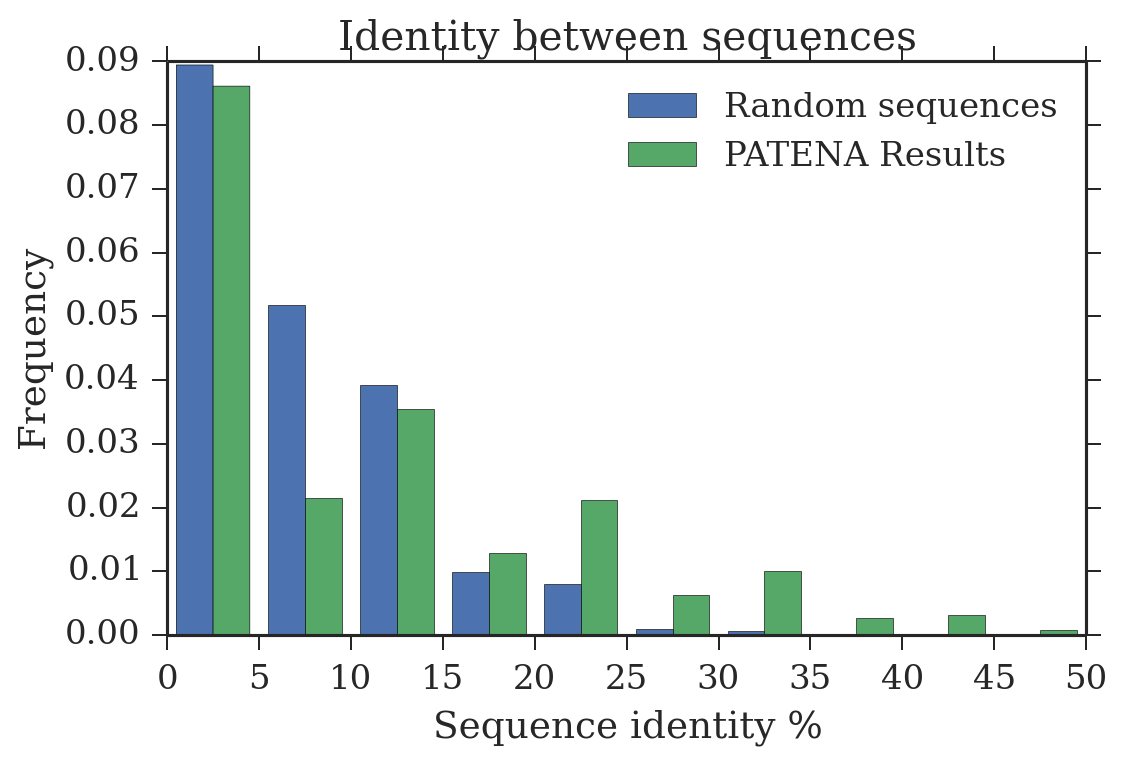
\includegraphics[width=200px,height=175px]{img/resultados/againstAll-random.png}
%    \caption{Histograma de identidad entre las secuencias resultantes y la secuencia inicial}
    \label{fig:identity-a}
    \end{subfigure}
  \hspace{20px}
  \begin{subfigure}[b]{200px}
  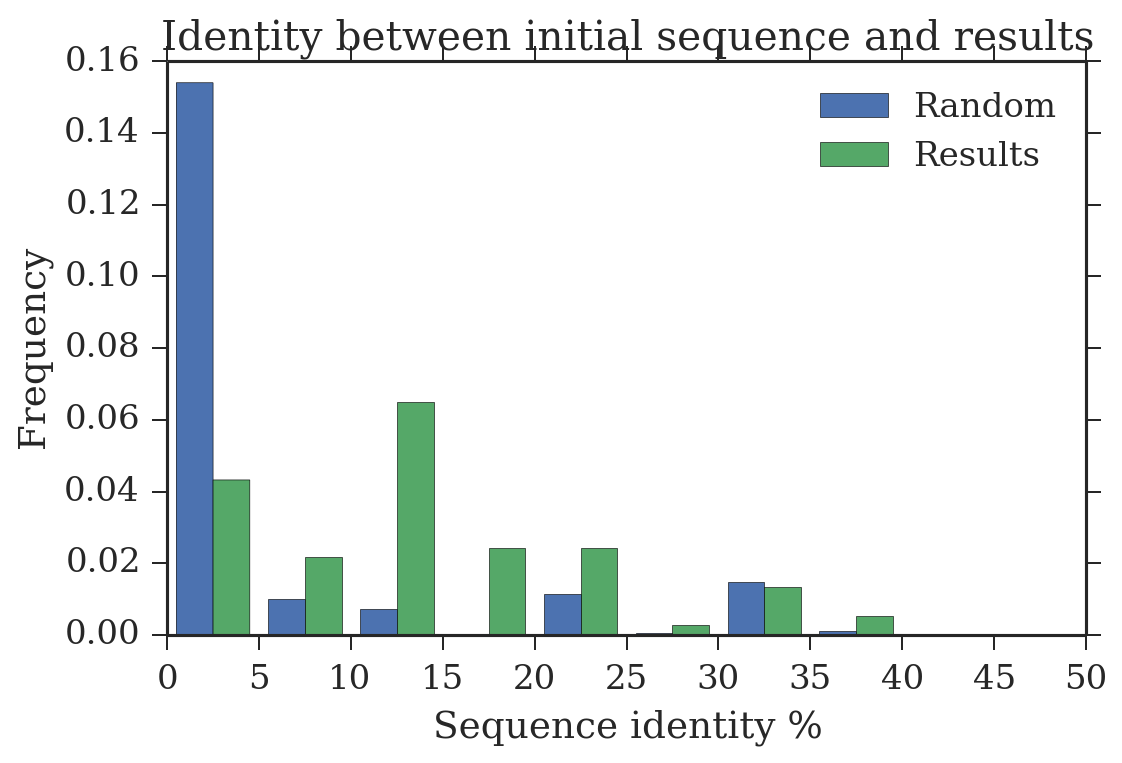
\includegraphics[width=200px,height=175px]{img/resultados/againstInitial-random.png}
    \label{fig:identity-b}
%     \caption{Histograma de identidad entre las secuencias resultantes entre si}
%     \caption{Identidad entre cada par posible de secuencias resultantes(74*74)}
  \end{subfigure}
  \caption{Histograma de identidad entre las secuencias resultantes entre si (izquierda) y entre éstas y la secuencia inicial (derecha)}
  \label{fig:identity}
\end{figure}



Sin embargo, este análisis de identidad global entre secuencias no permite conocer si la similitud se encuentra localizada en alguna posición especifica.
La extracción de un logo secuencial \cite{schneider1990sequence} permite obtener, a través de una representación gráfica, un análisis detallado de la similitud dentro de un conjunto de secuencias.
En la figura \ref{fig:logo} se muestra el logo obtenido a partir de los resultados correspondientes a las 74 corridas ejecutadas.
% La extracción de un logo secuencial a partir del conjunto de resultados permite analizar en detalle la similitud encontrada. 
% Un logo secuencial muestra, en una representación gráfica, la similitud dentro de un conjunto de secuencias \cite{schneider1990sequence}, 
% en este caso entre los resultados de las 74 corridas independientes (figura \ref{fig:logo}).


% los residuos que mas se repiten entre las secuencias resultantes son los correspondientes a las posiciones que inicialmente
Como se ve, la similitud entre los resultados se concentra en las posiciones que inicialmente 
poseían residuos de Glicina y Prolina (posiciones 9,18,19,21), y los residuos mas representados en estas posiciones son, justamente, los mismos que se encontraban en la secuencia inicialmente. 
Como vimos en el capítulo 1, estos son los residuos más encontrados en secuencias linkers tanto naturales como artificiales debido a sus propiedades fisicoquímicas, 
que permiten caracterizarlos como residuos que favorecen el desorden intrínseco en la conformación del polipéptido.
% Si revisamos los resultados del análisis de mutaciones para cada posición (figura \ref{fig:mutationPerSite}), veremos que, si bien no hay una diferencia significativa, 
% son justamente estas posiciones las que tienen menores porcentajes medio de mutación.
% Al parecer, estas posiciones mantienen un valor de puntaje bajo a lo largo de la ejecución y pueden, en algunos casos, finalizar la ejecución sin sufrir ninguna mutación. 
En estos casos, los residuos iniciales correspondientes a estas posiciones están más conservados en el diseño final.
Cabe aclarar que el grado de conservación encontrado es relativamente bajo ya que para secuencias de proteínas, como se describe en \cite{crooks2004weblogo}, la conservación toma valores entre $0$ y $log_2 20 \approx 4.32$.  
Por otro lado, el resto de las posiciones mantienen una gran diversidad que reflejan la heterogeneidad mostrada en las figuras previas.
% PONER QUE ES MUY BAJO EL VALOR DE BITS ()

\begin{figure}[htbp]
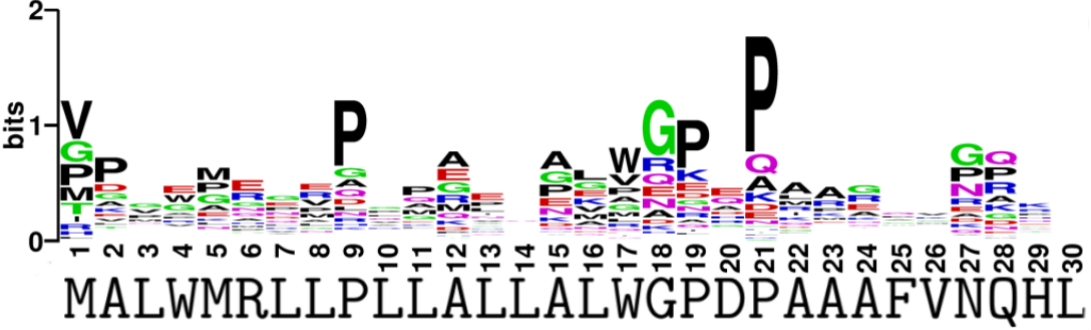
\includegraphics[width=\textwidth]{img/resultados/logoInitial.png}
\caption{\textbf{Representación gráfica de la similitud secuencial entre los resultados}. Debajo del logo se muestra la secuencia inicial a partir de la cual se obtuvieron los resultados. Figura obtenida utilizando \cite{crooks2004weblogo}}
\label{fig:logo}
\end{figure}
% por lo tanto, la similitud en estas posiciones parece ser producto de la falta de mutaciones.
% y por lo tanto que los residuos iniciales se mantienen intactos.
% Sin embargo, no hay una diferencia significativa en el porcentaje de mutaciones promedio que se aplican en estas posiciones, por lo que es posible que esta similitud puntual se deba que la
% La menor cantidad de mutaciones en estas posiciones se ve reflejada en la similitud secuencial entre los diseños resultantes.



% La diversidad obtenida es producto de la composición estandar que imponemos para la secuencia inicial y las mutaciones propuestas.
Por último queremos saber ahora si, además de la diversidad resultante que mostramos hasta aquí, estamos efectivamente minimizando el costo metabólico de los diseños obtenidos.
Es importante comprobar esto ya que el objetivo de utilizar la composición estándar extraída de Swissprot (detallado en \ref{seqInicial}) era obtener un correcto balance entre diversidad y costo metabólico asociado.
% Este es uno de los objetivos de utilizar la composición extraída de Swissprot (detallado en \ref{seqInicial}).
Para evaluarlo comparamos la frecuencia de cada aminoácido, extraída de los 74 resultados obtenidos, con la frecuencia esperada de acuerdo a la composición estándar que utilizamos en el método.
Los resultados, mostrados en el gráfico \ref{fig:frequencies}, muestran una correspondencia entre la frecuencia esperada y la resultante en este pequeño conjunto de resultados.
El caso que más se desvía de la correspondencia es el aminoácido Prolina, donde la frecuencia observada es considerablemente mayor que la esperada, lo cual es entendible si tenemos en cuenta las propiedades 
de este residuo comentadas previamente. Esta desviación es correspondiente, además, con la conservación encontrada en los resultados que se vió en la figura \ref{fig:logo}.





\begin{figure}[htbp]
\centering
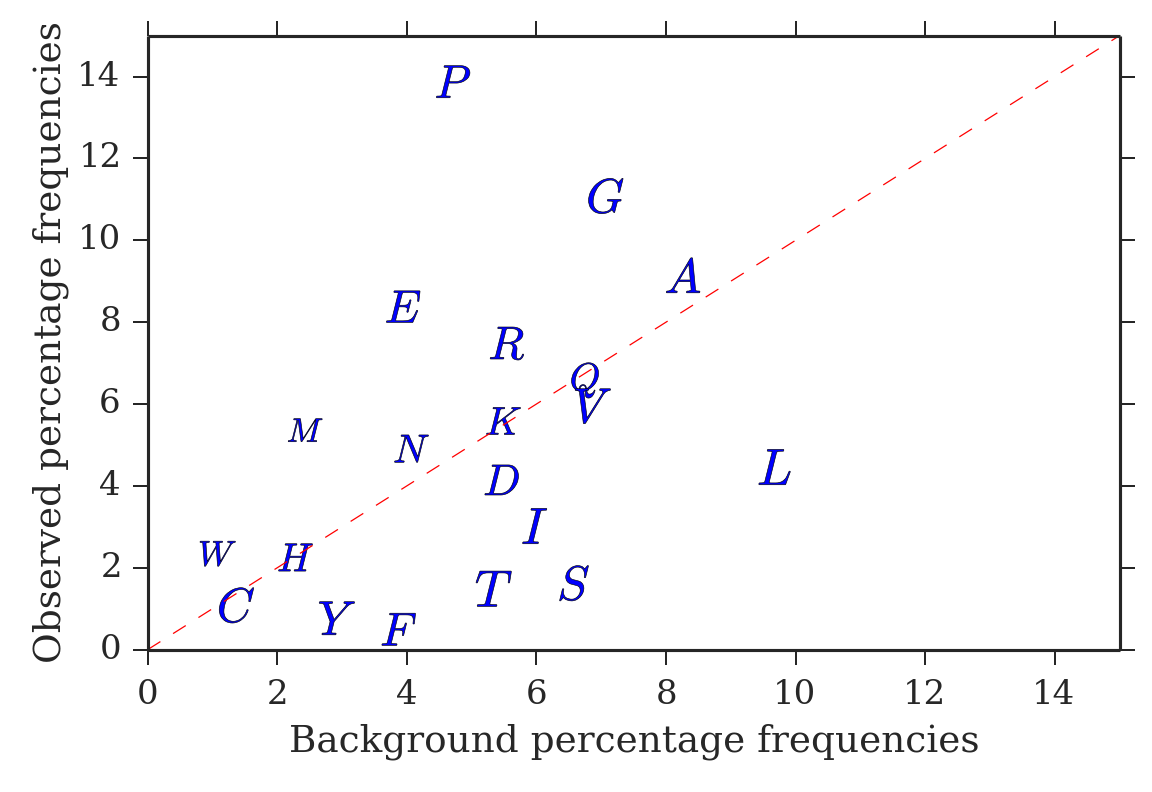
\includegraphics[width=0.70\textwidth]{img/resultados/frequenciesComparison.png}
\caption{\textbf{Comparación de frecuencias esperadas y frecuencias observadas en los diseños resultantes}}
\label{fig:frequencies}
\end{figure}
